\documentclass[times, utf8, diplomski, numeric]{fer}
\usepackage{booktabs}
\usepackage{url}
\usepackage{amsmath}
\usepackage{float}
\usepackage[]{algorithmic}
\usepackage[]{algorithm}
\usepackage{diagbox}

\renewcommand{\algorithmicfor}{\textbf{Za}}
\renewcommand{\algorithmicendfor}{\textbf{Kraj}}
\renewcommand{\algorithmicdo}{\textbf{Ponavljaj}}
\renewcommand{\algorithmicwhile}{\textbf{Sve dok}}
\renewcommand{\algorithmicendwhile}{\textbf{Kraj}}

\makeatletter
\renewcommand{\ALG@name}{Algoritam}
\makeatother

\allowdisplaybreaks

\begin{document}

\nocite{*}

% TODO: Navedite broj rada.
\thesisnumber{000}

% TODO: Navedite naslov rada.
\title{Detekcija sigurnosnih atributa prometnica u snimkama}

% TODO: Navedite vaše ime i prezime.
\author{Ivan Relić}

\maketitle

% Ispis stranice s napomenom o umetanju izvornika rada. Uklonite naredbu \izvornik ako želite izbaciti tu stranicu.
\izvornik

% Dodavanje zahvale ili prazne stranice. Ako ne želite dodati zahvalu, naredbu ostavite radi prazne stranice.
\zahvala{}

\tableofcontents

\chapter{Uvod}
Računalni vid vrlo je značajno područje umjetne inteligencije koje se bavi razumijevanjem slike, odnosno scene na slici. 
Vrlo popularna područja računalnog vida danas su klasifikacija (određivanje pripadnosti scene slike jednoj ili više predefiniranih klasa), semantička segmentacija (podjela slike u dijelove i pridjeljivanje klase svakom od tih dijelova), stereoskopska rekonstrukcija (određivanje 3D geometrije scene iz slika dobivenih parom kamera) te mnoga druga.
Važnost percepcije i razumijevanja okoline dovela je do toga da je računalni vid vrlo popularno područje umjetne inteligencije koje je u stalnom razvoju zbog svojih mnogih primjena.

Duboko učenje donijelo je veliku revoluciju na mnogim područjima umjetne inteligencije, pa tako i na području računalnog vida. 
Duboki modeli pomaknuli su margine najbolje ostvarenih rezultata na mnogim problemima. 
Primjerice,  na problemu klasifikacije slika iz skupa podataka ImageNet \citep{dataset:imagenet} u jednu od tisuću mogućih klasa, najmanja pogreška ostvarena dubokim modelom manja je od pogreške koju na tom skupu podataka ostvaruju ljudi \citep{article:delving_deep_into_rectifiers}. 
Upravo zbog vrlo dobrih rezultata koje duboki modeli ostvaruju, sve više zadataka u kojima ljudi lako griješe i koji su mentalno naporni povjeravaju se na obavljanje računalima.

Dobri rezultati dubokih modela na području računalnog vida svakako otvaraju mnoge primjene računala u praktičnim problemima. 
Jedan takav problem, kojim se ovaj rad bavi, jest inspekcija kvaliteta cesta. 
Organizacija iRAP \engl{International Road Assessment Programe} ima za cilj upravo inspekciju kvaliteta ceste pridruživanjem različitih sigurnosnih atributa dijelovima prometnica.
Zadatak se obavlja tako da se na temelju video sekvenci prometnica uz geolokacije pridružene video sekvencama određuje prisutnost sigurnosnog atributa na tom dijelu prometnice.
Na temelju prisutnih atributa moguće je procijeniti sigurnost promatranog dijela prometnice što je vrlo korisno.

Trenutno, pridruživanje atributa dijelovima prometnica obavljaju ljudi. 
Zadatak je vrlo naporan i skup te su moguće raznorazne greške -- greške uzrokovane subjektivnošću, greške uzrokovane nekonzistentnim pridruživanjem različitih osoba, greške uzrokovane umorom te mnoge druge.
Prednost korištenja dubokog modela za taj zadatak je njegova veća brzina, manja cijena i objektivnost u procjeni u odnosu na čovjeka.

Ovaj rad kroz nekoliko faza opisuje implementaciju dubokog modela koji je sposoban detektirati prisutnost sigurnosnog atributa u video snimci.
Prvi dio rada opisuje korišteni skup podataka -- postupak njegovog prikupljanja te korištenje za učenje dubokog modela.
Drugi dio rada opisuje korištene metode i modele koji na temelju učenja na skupu podataka ostvaruju željenu funkciju koju možemo primijeniti na konkretan problem.
Završni dio rada opisuje provedene eksperimente i dobivene rezultate prilikom korištenja dubokog modela za problem detekcije sigurnosnih atributa u snimkama.


\chapter{Skupovi podataka i njihovo korištenje} \label{chapter:skupovi_podataka}

Sustav koji rad opisuje temelji se na prepoznavanju prisutnosti atributa na prometnicama. 
Prepoznavanje prisutnosti atributa možemo okarakterizirati kao binarnu klasifikaciju čiji konačni izlaz nam govori je li atribut prisutan u sceni ili nije.

Modeli dubokog učenja danas uspješno rješavaju probleme klasifikacije. Rješavanje takvog problema temelji se na odabiru prikladnog modela uz dovoljan broj označenih podataka. 
Ključna stvar prilikom rješavanja problema klasifikacije jest izvlačenje znanja iz označenih podataka koje model koristi. Takav postupak nazivamo nadziranim učenjem \citep{book:deeplearningbook}. 
Prilikom učenja ustvari se korigiraju slobodni parametri modela koji ostvaruju željenu funkciju preslikavanja.

Skup podataka možemo podijeliti na 3 podskupa koji imaju različite uloge:
\begin{itemize}
 \item podskup za učenje -- podskup koji se koristi za korekciju slobodnih parametara modela
 \item podskup za validaciju -- podskup koji se koristi za korekciju hiperparametara, odnosno za provjeru sposobnosti generalizacije modela
 \item podskup za testiranje -- podskup koji se koristi za konačno ispitivanje performanse naučenog modela
\end{itemize}


\section{Video snimke projekta FTTS iRAP}

Baza video snimaka prometnica sa stranice \citep{url:ftts_irap} korištena je kao osnova za kreiranje skupa podataka. 
Video snimke snimljene su automobilom koji se kretao po engleskim autocestama.

Stranica \citep{url:ftts_irap} nudi sučelje u kojem je moguće segmentima prometnica pridruživati ranije spomenute sigurnosne atribute. 
Standard organizacije iRAP propisuje 78 atributa \citep{man:ftts_irap_attributes} koje je moguće pridružiti segmentima prometnica.
Pojedine video snimke je moguće preuzeti uz pripadajuće informacije o geolokaciji scena.

Sustav koji ovaj rad opisuje koristi video snimke s navedene stranice za učenje. Konkretno, kako je riječ o binarnoj klasifikaciji, potrebni su nam označeni podaci. 
Atribut koji sustav prepoznaje jest pripajanje \engl{merge lane}. Kako je riječ o video sekvencama s engleskih cesta, pripajanja koja se prepoznaju bit će s lijeve strane.
Definicija atributa pripajanje prema \citep{man:ftts_irap_coding_manual} jest sljedeća -- promet koji prilazi sa strane pripaja se preko linije za pripajanje na cestu kojoj se atribut dodjeljuje.

\begin{figure}[H]
\centering
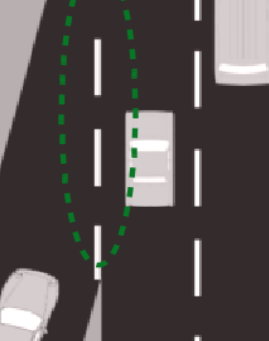
\includegraphics[scale=0.75]{images/merge_lane.png}
\caption{Simbolički prikaz pripajanja, preuzeto i prerađeno iz \citep{man:ftts_irap_coding_manual}}
\label{img:merge_lane_symbolic}
\end{figure}

\noindent Slika \ref{img:merge_lane_symbolic} simbolički prikazuje što se smatra pripajanjem prilikom pridjeljivanja sigurnosnog atributa pripajanja.
Iz video snimaka kreirana su dva tipa skupova podataka:
\begin{itemize}
 \item ručno označen skup podataka
 \item skup podataka označen konzistentno s podacima projekta FTTS iRAP
\end{itemize}
U nastavku je opisan način kreiranja i uporaba pojedinih tipova skupova podataka.

\section{Ručno označen skup podataka}
Početna ideja bila je, neovisno o pridruženim atributima pripajanja sa stranice \citep{url:ftts_irap}, ručno označiti pripajanja. 

Dubokim modelima je, kao i ljudima, lakše izlučiti znanje iz podataka ukoliko u njima postoje diskriminativne značajke koje mogu odrediti pripadnost određenoj klasi.
Dodjeljivanje oznaka prisutnosti atributa pripajanja prometnoj sceni iz tog se razloga vodilo tom mišlju -- scene na kojima su prisutne karakteristične, diskriminativne značajke koje bi mogle odrediti prisutnost atributa pripajanja označene su kao pozitivne, odnosno scene na kojima je atribut prisutan, dok su ostale označene kao negativne, odnosno scene na kojima atribut nije prisutan.

\begin{figure}[H]
\centering
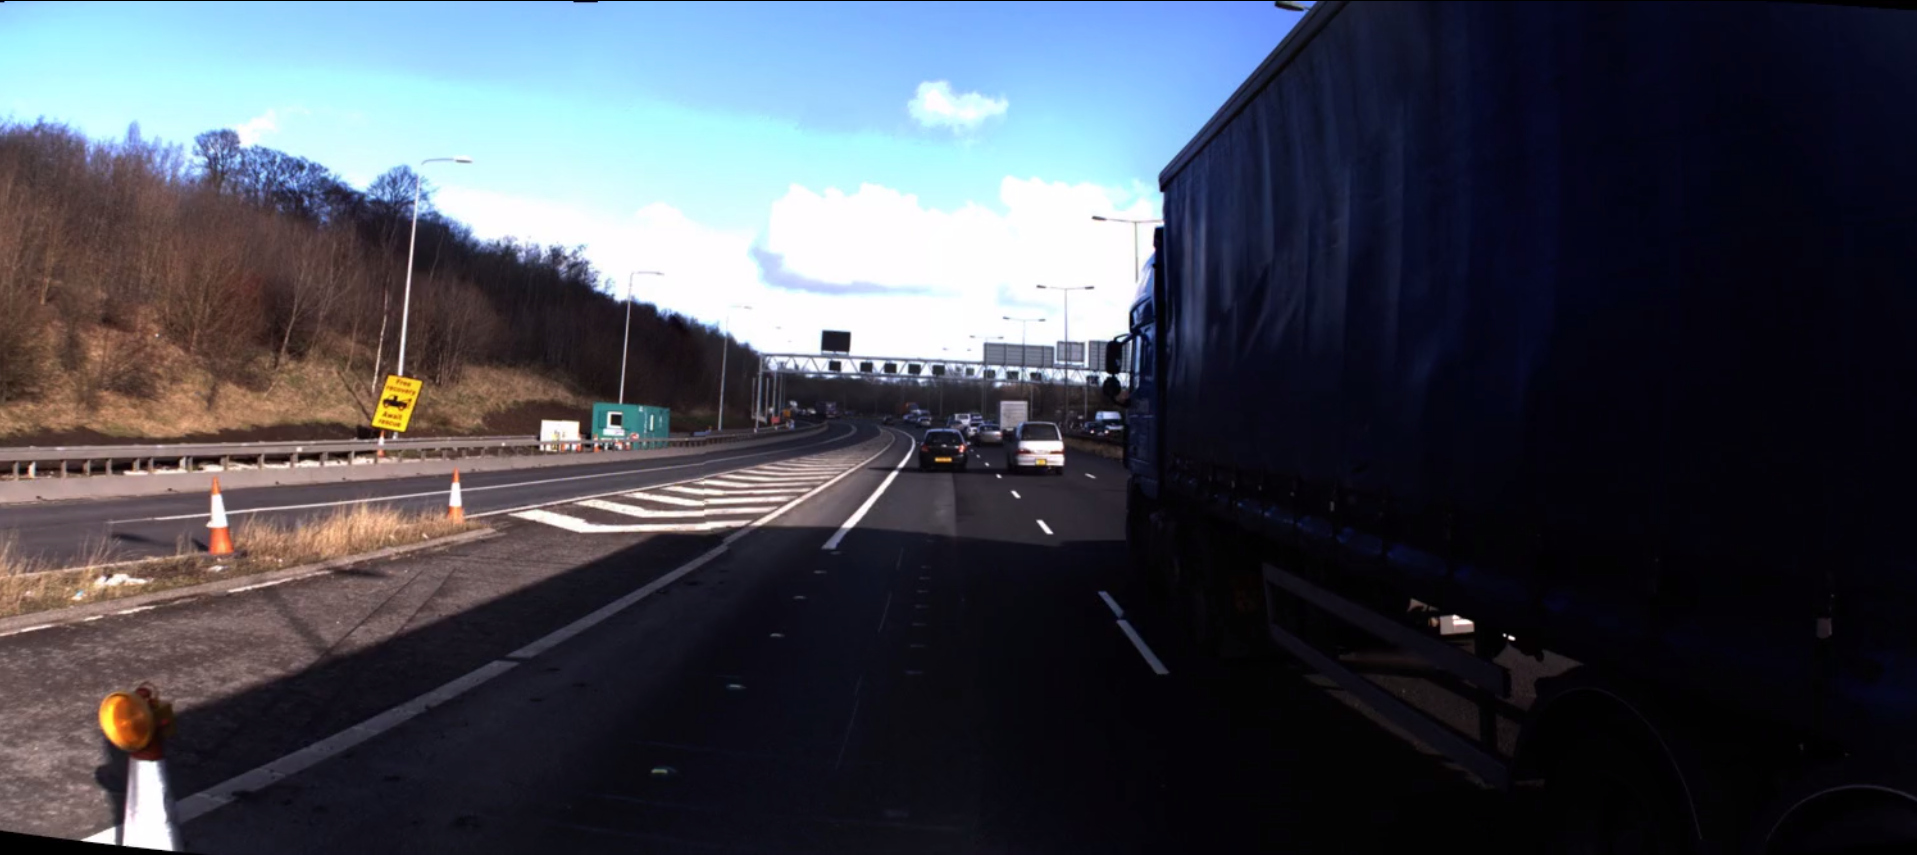
\includegraphics[scale=0.15]{images/hand_labeled_positive.png}
\caption{Prikaz ručno označene scene na kojoj je atribut pripajanja prisutan, preuzeto s \citep{url:ftts_irap}}
\label{img:hand_labeled_positive}
\end{figure}

\noindent Slika \ref{img:hand_labeled_positive} prikazuje ručno označenu pozitivnu sliku. 
Na slici su vidljive karakteristične bijele trake u uzorku koji bi potencijalno mogao biti diskriminativan prilikom donošenja odluke modela o prisutnosti atributa pripajanja.

\begin{figure}[H]
\centering
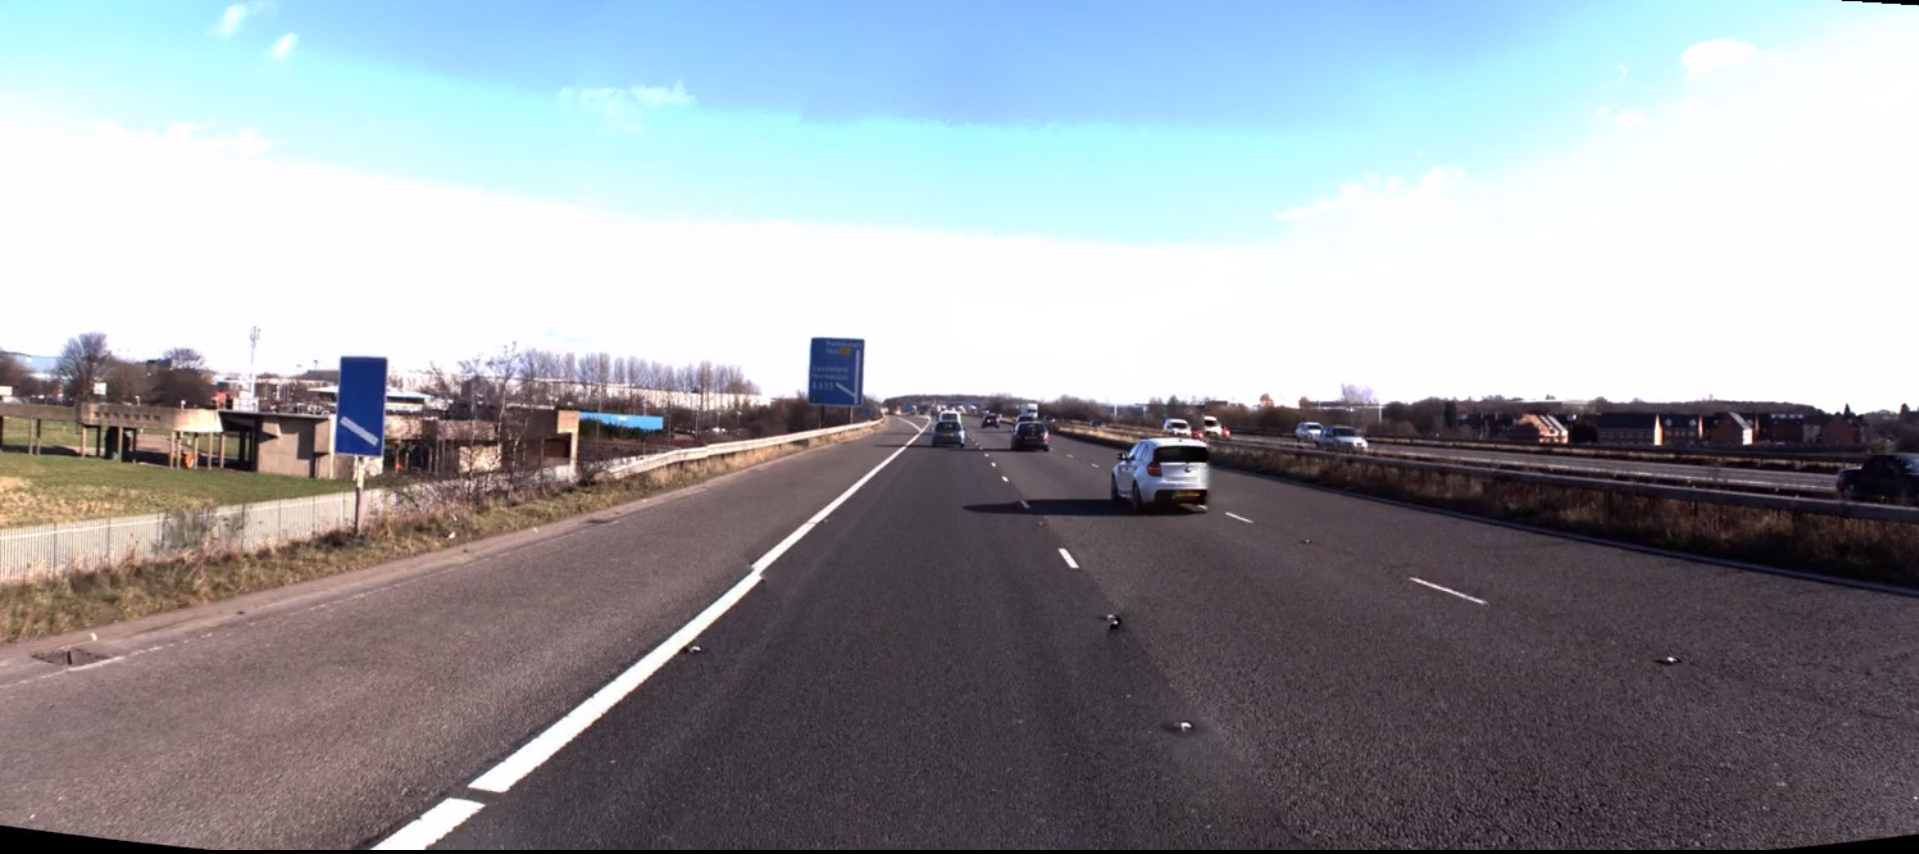
\includegraphics[scale=0.15]{images/hand_labeled_negative.png}
\caption{Prikaz ručno označene scene na kojoj atribut pripajanja nije prisutan, preuzeto s \citep{url:ftts_irap}}
\label{img:hand_labeled_negative}
\end{figure}

\noindent Slika \ref{img:hand_labeled_negative} prikazuje ručno označenu negativnu sliku.
Vidljiv je izostanak karakterističnih bijelih traka na cijeloj sceni.

Ručno označen skup podataka dobiven je obradom 7 videa preuzetih sa stranice \citep{url:ftts_irap}. 
Ukupan broj dobivenih označenih slika s raspodjelom u podskupove je sljedeći:
\begin{itemize}
 \item podskup za učenje -- 1796 slika, od toga 898 pozitivnih
 \item podskp za validaciju -- 626 slika, od toga 313 pozitivnih
 \item podskup za testiranje -- 594 slike, od toga 297 pozitivnih
\end{itemize}

\noindent Skup je kreiran na način da se iz svake video sekvence uzorkuju pozitivni primjeri (primjeri na kojima je prisutna diskriminativna značajka atributa pripajanja) te se zatim uzorkuje isti broj negativnih primjera na kojima diskriminativna značajka karakterističnog bijelog uzorka nije prisutna.

\section{Skup podataka označen konzistentno s projektom FTTS iRAP}
Kako je glavni cilj rada razviti sustav koji bi mogao automatski određivati prisutnost sigurnosnog atributa na prometnoj sceni, za učenje je potrebno kreirati takav skup podataka koji je označen konzistentno s pravilima koja propisuje iRAP.

U dogovoru s kreatorima stranice \citep{url:ftts_irap}, izvučeni su podaci geolokacije svih segmenata prometnica na kojima je prisutan atribut pripajanja. 
Segmenti na kojima se određuje je li sigurnosni atribut prisutan ili nije dugački su $10$m.
Također, moguće je i otvoriti video snimku koja prikazuje trenutak kada započinje segment s atributom pripajanja.

\begin{figure}[H]
\centering
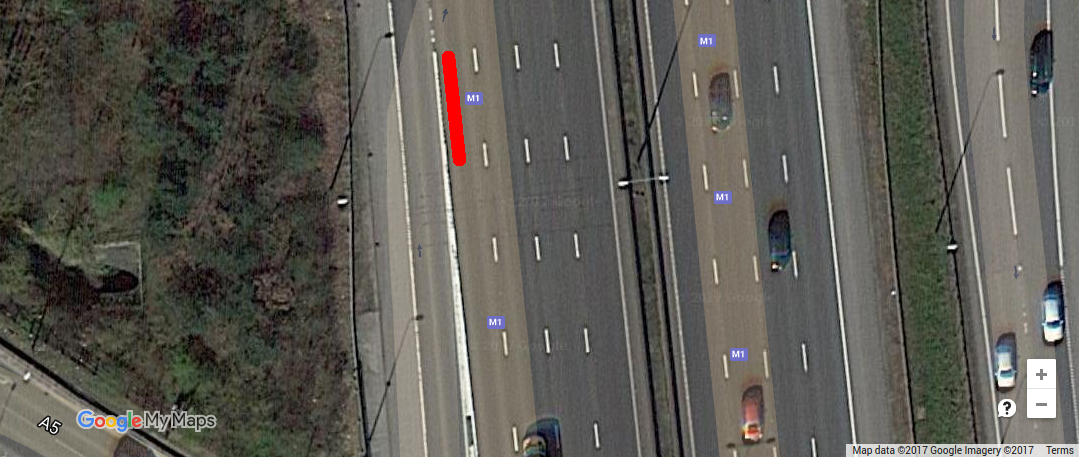
\includegraphics[scale=0.35]{images/sattelite_merge_lane_irap.png}
\caption{Prikaz satelitske snimke s označenim segmentom atributa pripajanja, preuzeto s \citep{url:google_maps}}
\label{img:sattelite_merge_lane_irap}
\end{figure}

Promotrimo sliku \ref{img:sattelite_merge_lane_irap}. Na slici je crvenom linijom označen segment koji je na stranici \citep{url:ftts_irap} prema pravilima koje propisuje iRAP označen kao pripajanje. 
Već sa satelitske snimke je vidljivo kako bi moglo biti problema prilikom učenja zbog nedostatka diskriminativnih značajki koje bi mogle olakšati raspoznavanje pripajanja.

\begin{figure}[H]
\centering
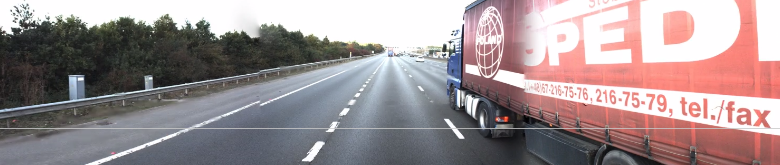
\includegraphics[scale=0.5]{images/video_merge_lane_irap.png}
\caption{Prikaz video snimke s označenim segmentom atributa pripajanja, preuzeto s \citep{url:ftts_irap}}
\label{img:video_merge_lane_irap}
\end{figure}

\noindent Slika \ref{img:video_merge_lane_irap} prikazuje isječak iz video snimke u trenutku kada započinje segment označen kao pripajanje. 
Iz same slike je vrlo teško odrediti da je u tom trenutku prisutan atribut pripajanja.

Problem nedostatka informacije možemo riješiti tako da odluku ne temeljimo na jednoj slici nego na sekvenci slika koje su prethodile trenutnoj. 
Koristeći sekvencu slika koja prethodi slici označenoj kao početak segmenta označenog kao pripajanje, model će biti u mogućnosti lakše donijeti odluku zbog prisutnosti diskriminativne značajke (karakteristične bijele trake u uzorku).
Prisutnost diskriminativne značajke u sekvenci koja prethodi početku pripajanja vidljiva je i iz satelitske snimke.
Skup podataka označen konzistentno s projektom FTTS iRAP iz tog razloga ne sadrži statične, pojedinačne slike nego sekvence slika.

Skup podataka označen konzistentno s projektom FTTS iRAP dobiven je obradom 100 videa preuzetih sa stranice \citep{url:ftts_irap}. 
Ukupan broj dobivenih označenih sekvenci s raspodjelom u podskupove je sljedeći:
\begin{itemize}
 \item podskup za učenje -- 7554 sekvenci, od toga 3777 pozitivnih
 \item podskp za validaciju -- 1720 sekvenci, od toga 860 pozitivnih
 \item podskup za testiranje -- 1642 sekvenci, od toga 821 pozitivnih
\end{itemize}

\noindent Skup je kreiran na način da se iz svake video sekvence uzorkuju pozitivni primjeri na sljedeći način: 
\begin{itemize}
 \item odrede se rasponi sličica video snimke koji su prema stranici \citep{url:ftts_irap} označeni kao pozitivni (sadrže atribut pripajanja)
 \item za svaku sličicu označenu kao pozitivnu uzorkuje se i nekoliko sličica unatrag koje će zajedno činiti jednu pozitivnu sekvencu
\end{itemize}

\noindent Na sličan način uzorkuje se i jednak broj negativnih primjera za one sličice za koje je prema stranici \citep{url:ftts_irap} označeno da ne sadrže atribut pripajanja.
Cjelokupni postupak kreiranja skupa podataka uz konkretne podatke o duljini sekvence bit će dan u nastavku rada.

\chapter{Korištene metode, modeli i postupci prilikom oblikovanja sustava}
Sustav koji ovaj rad opisuje temelji se na algoritmima dubokog učenja. 
Zadatak koji je potrebno riješiti jest binarna klasifikacija, odnosno određivanje je li atribut pripajanja prisutan u prometnoj sceni.
Model koji rješava zadatak tada možemo prikazati sljedećom funkcijom:

\begin{equation}
 \mathbf{y} = f^*(\mathbf{x}; \boldsymbol{\phi}),
\end{equation}

\noindent gdje je $f^*$ funkcija koju želimo naučiti koristeći skup podataka. Argumenti funkcije $f^*$ su ulazni vektor podataka $\mathbf{x}$ te skup slobodnih parametara, $\boldsymbol{\phi}$.
Vrijednost funkcije $f^*$, odnosno $\mathbf{y}$ predstavlja upravo željenu informaciju koja nas zanima -- vjerojatnost da je atribut pripajanja prisutan, odnosno vjerojatnost da atribut pripajanja nije prisutan na prometnoj sceni koja je predstavljena kao ulazni vektor podataka $\mathbf{x}$.

Modeli dubokog učenja pretpostavljaju kompozitnu strukturu ulaznih podataka -- npr. čovjek je građen od glave i tijela, glava je građena od očiju, usta, nosa i ušiju, oči su građene od rožnice, zjenice i šarenice, i td.
Iz tog razloga se nad ulaznim podacima obavljaju višestruke linearne i nelinearne operacije \citep{pdf:duboko_0}.
Funkciju $f^*$ stoga možemo prikazati i na sljedeći način:
$f^*(\mathbf{x}; \boldsymbol{\phi})=f^{(n)}(f^{(n-1)}(...f^{(2)}(f^{(1)}(\mathbf{x}, \boldsymbol{\phi}), \boldsymbol{\phi}), \boldsymbol{\phi}), \boldsymbol{\phi})$ \citep{book:deeplearningbook}.
Pojedine funkcije $f^{(i)}$ predstavljaju slojeve dubokog modela koje obavljaju različite operacije.

Ocjenu prikladnosti funkcije $f^*$ sa slobodnim parametrima $\boldsymbol{\phi}$ možemo mjeriti funkcijom gubitka. 
Funkcija gubitka nam govori koliko dobro naša funkcija sa slobodnim parametrima aproksimira stvarna preslikavanja koja su definirana na skupu podataka za učenje.

Učenje modela, odnosno optimizacija, tada se svodi na pretraživanje za onim skupom slobodnih parametara koji će minimizirati funkciju gubitka nad skupom podataka za učenje.
Optimizacijski postupak koji se koristi je gradijentni spust nad funkcijom gubitka koju deriviramo po slobodnim parametrima modela.

Nastavak rada opisuje korištenu funkciju gubitka, optimizacijsku metodu za učenje modela te tipične slojeve dubokih modela koji se koriste za primjenu u računalnom vidu.
Opisane su i konkretne arhitekture koje su se koristile prilikom provođenja eksperimenata te detaljni postupci kojima su generirani skupovi podataka.

\section{Unakrsna entropija kao funkcija gubitka}
Unakrsna entropija kao funkcija gubitka izvodi se kao negativni logaritam izglednosti modela nad podacima. Učenjem želimo maksimizirati izglednost parametara nad nekim podacima za učenje, odnosno želimo parametre modela za koje je najizglednije da minimiziraju razliku između funkcije $f$ koju aproksimiramo i aproksimirane funkcije modela $f^*$.

Pretpostavke za izvod unakrsne entropije kao funkcije gubitka su sljedeće:
\begin{itemize}
 \item zadatak koji rješavamo jest zadatak klasifikacije slike u jednu od $k$ različitih klasa
 \item izlazni vektor je dimenzionalnosti $k$ i označava međusobno zavisne vjerojatnosti da ulazni podatak pripada svakoj od $k$ klasa
 \item podaci za učenje su izvučeni iz iste razdiobe i međusobno su nezavisni
\end{itemize}

\noindent Izvedimo unakrsnu entropiju kao funkciju gubitka iz logaritma izglednosti modela nad podacima:
\begin{align}
 C &= - \ln \mathcal{L}(\boldsymbol{\phi}, \mathcal{D}) = - \ln (p_{model}(\mathbf{x}, \mathbf{y} | \mathcal{D}, \boldsymbol{\phi})) \nonumber \\
 &= - \ln \prod_{\mathbf{x} \in \mathcal{D}} \prod_{j=1}^{k} (p_{model}(\mathbf{y}_k | \mathbf{x}, \mathcal{D}, \boldsymbol{\phi})) p_{model}(\mathbf{x})\nonumber \\
 &= - \sum_{\mathbf{x} \in \mathcal{D}} \sum_{j=1}^{k} \ln (f_j^*(\mathbf{x})^{f_j(\mathbf{x})}  (1 - f_j^*(\mathbf{x}))^{(1 - f_j(\mathbf{x}))}) \nonumber \\
 &= - \sum_{\mathbf{x} \in \mathcal{D}} \sum_{j=1}^{k} (\ln f_j^*(\mathbf{x})^{f_j(\mathbf{x})} + \ln (1 - f_j^*(\mathbf{x}))^{(1 - f_j(\mathbf{x}))}) \nonumber \\
 &= - \sum_{\mathbf{x} \in \mathcal{D}} \sum_{j=1}^{k} (f_j(\mathbf{x}) \ln f_j^*(\mathbf{x}) + (1 - f_j(\mathbf{x})) \ln (1 - f_j^*(\mathbf{x}))) \label{eq:neg_log_likelihood}
\end{align}
gdje je $k$ dimenzionalnost izlaznog vektora, $f_j(\mathbf{x})$ je stvarni izlaz (0 ili 1), a $f_j^*(\mathbf{x})$ je vrijednost $j$-te komponente izlaznog vektora za primjer $\mathbf{x}$ iz skupa podataka za učenje.
Vjerojatnost $p_{model}( \mathbf{y} | \mathbf{x},\mathcal{D}, \boldsymbol{\phi})$ predstavlja vjerojatnost oznake primjera. Kako su izlazi modela iz intervala $\left[ 0, 1\right]$,
navedenu vjerojatnost možemo zapisati kao $f_j^*(\mathbf{x})^{f_j(\mathbf{x})}  (1 - f_j^*(\mathbf{x}))^{(1 - f_j(\mathbf{x}))}$.
Član $p_{model}(\mathbf{x})$ možemo slobodno zanemariti prilikom definiranja funkcije gubitka jer ne ovisi o vrijednostima parametara $\boldsymbol{\phi}$ \citep{seminar:rela}.

\section{Gradijentni spust}

Izračun nove vrijednosti parametra $\phi$ funkcije $y$ čija se vrijednost minimizira definiran je kao:
\begin{equation}
 \phi_{n+1} = \phi_n - \psi \cfrac{\partial y}{\partial \phi}, \label{eq:gradient_descent}
\end{equation}
gdje je $\psi$ pozitivna, uobičajeno mala konstanta koja kontrolira faktor korekcije parametra.

\noindent U slučaju učenja dubokog modela, izraz \ref{eq:gradient_descent} možemo zapisati kao:
\begin{equation}
 \boldsymbol{\phi}_{n+1} = \boldsymbol{\phi}{_n} - \eta \cfrac{\partial C}{\partial \boldsymbol{\phi}}, \label{eq:gradient_descent_neural}
\end{equation}
gdje je $\boldsymbol{\phi}$ skup slobodnih parametara modela, $\eta$ je parametar algoritma učenja koji nazivamo stopa učenja \engl{learning rate} kojim definiramo koliko će se po iznosu mijenjati parametri prilikom učenja.
Funkcija koju optimiramo je funkcija gubitka, $C$.

Postoje različite varijante osnovnog algoritma za korekciju parametara modela. 
Korekciju parametara moguće je vršiti akumulirajući gradijent parametara po svim primjerima iz skupa za učenje, gdje govorimo o stvarnom gradijentu nad funkcijom gubitka, $C$. 
Akumulirani gradijent se zatim koristi za korekciju parametara prema izrazu \ref{eq:gradient_descent_neural}. U tom slučaju govorimo o klasičnom gradijentnom spustu.

Varijanta u kojoj se gradijent izračunat u svakom primjeru odmah koristi za korekciju parametara naziva se stohastički gradijentni spust. 
Stohastičnost varijante očituje se u tome što ustvari ne računamo stvarni gradijent funkcije gubitka $C$, nego funkcije $C_\mathbf{x}$ koja definira gubitak nad jednim određenim primjerom $\mathbf{x}$ iz skupa za učenje.
Stohastički gradijentni spust pokazuje bolju otpornost na zaglavljivanje u lokalnim optimumima, ali i brže učenje zbog češće korekcije parametara.

Varijanta u kojoj se gradijent akumulira nad određenim brojem primjera i zatim se koristi za korekciju parametara naziva se grupni \engl{batched} gradijentni spust \citep{seminar:rela}.

\subsection{Adam optimizator}
Za potrebe učenja modela korištenog u ovom radu korišten je Adam optimizator. 
Adam optimizator je modificirana varijanta klasičnog algoritma gradijentnog spusta koja je robusnija i daje bolje rezultate \citep{article:adam}.

Adam optimizator, za razliku od klasičnog algoritma gradijentnog spusta kombinira dvije napredne tehnike prilikom korekcije parametara. 
Uvode se metode momenta i adaptivnog pomaka što pospješuje učenje dubokih modela.

Metoda momenta pomaže ubrzanju učenja na način da prilikom korekcije parametara modela u obzir uzima i iznos prethodne korekcije --- samo ime i analogija dolaze iz područja fizike pa metodu možemo poistovjetiti s tromosti tijela.
Korekcija parametara se, u odnosu na izraz \ref{eq:gradient_descent_neural}, definira na sljedeći način:
\begin{align}
\mathbf{v}_{n+1} &= \alpha \mathbf{v}_{n} - \eta \cfrac{\partial C}{\partial \boldsymbol{\phi}} \\
 \boldsymbol{\phi}_{n+1} &= \boldsymbol{\phi}_n + \mathbf{v}_{n+1}
\end{align} 
Parametar $\alpha$ određuje jačinu momenta, odnosno utjecaj prethodne korekcije na trenutnu korekciju i njegov iznos bi u ranijim fazama učenja trebao biti niži, a u kasnijima viši jer tada želimo što usmjereniju pretragu.
Osim ubrzanja učenja, momentum pospješuje i otpornost na zaglavljivanje u lokalnim optimumima jer je moguće ``preskočiti'' lokalni optimum u koji bismo inače zaglavili slijepo prateći samo iznos gradijenta \citep{book:deeplearningbook} \citep{seminar:rela}.

Metoda adaptivnog pomaka pretpostavlja da je stabilnost gradijenta ovisna o svakoj komponenti parametara koji se optimiraju pa je smisleno koristiti zasebne stope učenja za svaku od njih i automatski ih adaptirati kroz postupak učenja.
Konačan efekt jest da će se komponente parametara čije su parcijalne derivacije po funkciji gubitka vrlo visokih vrijednosti korigirati sa značajno manjim stopama učenja, a komponente parametara čije su parcijalne derivacije po funkciji gubitka relativno niskih vrijednosti, korigirat će se većim stopama učenja \citep{book:deeplearningbook} \citep{seminar:rela}.

Adam optimizator kombinira ove dvije metode i optimiranje parametara definira se na sljedeći način:
\begin{align}
 \text{inicijalne vrijednosti}&: \nonumber \\
 t_0 &= 0 \nonumber \\
 \mathbf{m}_0 &= \vec{0} \nonumber \\
 \mathbf{v}_0 &= \vec{0} \nonumber  \\
 \text{osvježavanje parametara}&: \nonumber \\
 \mathbf{g}_t &= \cfrac{\partial C}{\partial \boldsymbol{\phi}_t}  \nonumber \\
 \mathbf{m}_t &= \beta_1 \mathbf{m}_{t-1} + (1 - \beta_1) \mathbf{g}_t \nonumber \\
 \mathbf{v}_t &= \beta_2 \mathbf{v}_{t-1} + (1 - \beta_2) \mathbf{g}_t^2 \nonumber \\
 \hat{\mathbf{m}_t} &= \cfrac{\mathbf{m}_t}{1 - \beta_1^t} \nonumber \\
 \hat{\mathbf{v}_t} &= \cfrac{\mathbf{v}_t}{1 - \beta_2^t} \nonumber \\
 \boldsymbol{\phi}_{t+1} &= \boldsymbol{\phi}_t - \eta \cfrac{\hat{\mathbf{m}_t}}{\sqrt{\hat{\mathbf{v}_t}} + \epsilon} \nonumber,
\end{align}
gdje je $t$ vremenski korak koji se inkrementira sa svakom korekcijom parametara, $\eta$ je stopa učenja, $\beta_1$ i $\beta_2$ su faktori korišteni za
eksponencijalni pomični prosjek \engl{exponential moving average}. Preporučene vrijednosti su $\beta_1=0.9$ i $\beta_2=0.999$ \citep{article:adam}.
Parametar $\epsilon$ služi za izbjegavanje dijeljenja s nulom i postavlja se na vrlo malu vrijednost (npr. $10^{-8}$).


\subsection{Prenaučenost modela}

Slojevi u dubokim modelima često imaju vrlo velik broj parametara što može dovesti do problema prenaučenosti.
Vrlo česta regularizacijska metoda koja nastoji spriječiti prenaučenost jest regularizacija metodom smanjenja težina \engl{weight decay}.
Regularizacija metodom smanjenja težina mijenja funkciju gubitka koja se optimira tako da uvodi član ovisan o normi parametara, i to na sljedeći način:
\begin{equation}
 C^* = C + \lambda p(\boldsymbol{\phi}),
\end{equation}
gdje je $C^*$ nova funkcija gubitka koju optimiramo, $C$ je originalna funkcija gubitka, $p(\boldsymbol{\phi})$ predstavlja funkciju norme nad parametrima $\boldsymbol{\phi}$, a $\lambda$ je regularizacijski faktor.
Faktor $\lambda$ određuje utjecaj regularizacije -- što je on veći, regularizacija je jača i dobivamo jednostavnije modele koji nisu skloni prenaučenosti.

Motivacija za korištenje regularizacije metodom smanjenja težina leži u tome da će funkcije neuronskih mreža koje imaju niže vrijednosti težina biti zaglađenije, odnosno imat će nižu varijancu što je poželjno za bolju generalizaciju.
Obično se prilikom regularizacije parametri koji modeliraju pomak ne regulariziraju jer je na njih dovedena konstantna vrijednost ulaza pa samim time utječu samo na pomak unutar prostora \citep{seminar:rela}.

Često korištene funkcije norme $p(\boldsymbol{\phi})$ za vektor slobodnih parametara dimenzionalnosti $n$ jesu:
\begin{description}
 \item [L1 norma] $p(\boldsymbol{\phi})=\sum_{i=1}^n \left| \boldsymbol{\phi}_i \right|$ --- L1 \engl{Lasso} regularizacija
 \item [L2 norma] $p(\boldsymbol{\phi})=\sqrt{\sum_{i=1}^n  \boldsymbol{\phi}_i^2 }$ --- L2 \engl{Ridge} regularizacija
 
\end{description}

\section{Tipični slojevi dubokih modela za primjenu u računalnom vidu}
Duboki modeli koji se koriste za primjenu u računalnom vidu tipično su građeni od nekoliko različitih slojeva koji imaju različite uloge.
Slojevi obavljaju različite operacije nad podacima i tako ostvaruju željenu konačnu funkcionalnost koja je potrebna da se obavi neki zadatak.

\subsection{Potpuno povezani sloj}
Operacija koju obavlja potpuno povezani sloj definirana je na sljedeći način:

\begin{equation}
 \mathbf{y}=g(\mathbf{W}\mathbf{x}),
\end{equation}

\noindent gdje je $\mathbf{x}$ vektor ulaznih podataka, $g$ je aktivacijska funkcija, a  $\mathbf{y}$ je vektor izlaznih podataka. 
Vektor ulaznih podataka obično se proširuje na oblik $\mathbf{x} = \begin{bmatrix} 1 & x_1 & x_2 & ... & x_n \end{bmatrix}^T$.
Vrijednost $\mathbf{x}_1$ se fiksno postavlja na vrijednost $1$ iz razloga što želimo dozvoliti da model modelira pomak parametrima prvog stupca matrice $\mathbf{W}$.
Primjetimo kako će upravo dimenzionalnost matrice $\mathbf{W}$ određivati dimenzionalnost vektora izlaznih podataka.

Aktivacijska funkcija $g$ djeluje po elementima vektora dobivenog operacijom matričnog množenja matrice $\mathbf{W}$ i vektora ulaznih podataka $\mathbf{x}$.
Tipično se koriste nelinearne aktivacijske funkcije kako bismo dobili veću ekspresivnost dubokog modela.
Postoje različite aktivacijske funkcije koje se u praksi koriste. U nastavku su opisane neke od njih.

\subsubsection{Sigmoidalna aktivacijska funkcija}
Sigmoidalna aktivacijska funkcija i njena derivacija definirane su kao: 
\begin{align}
 g^{(i)}_j(\mathbf{x})&=\cfrac{1}{1+e^{-\alpha x_j}}, \\
 \frac{dg^{(i)}(\mathbf{x})}{d\mathbf{x}}&=\alpha g^{(i)}(\mathbf{x}) (1-g^{(i)}(\mathbf{x})) \label{eq:sigmoid_derivative}
\end{align}

\begin{figure}[H]
\centering
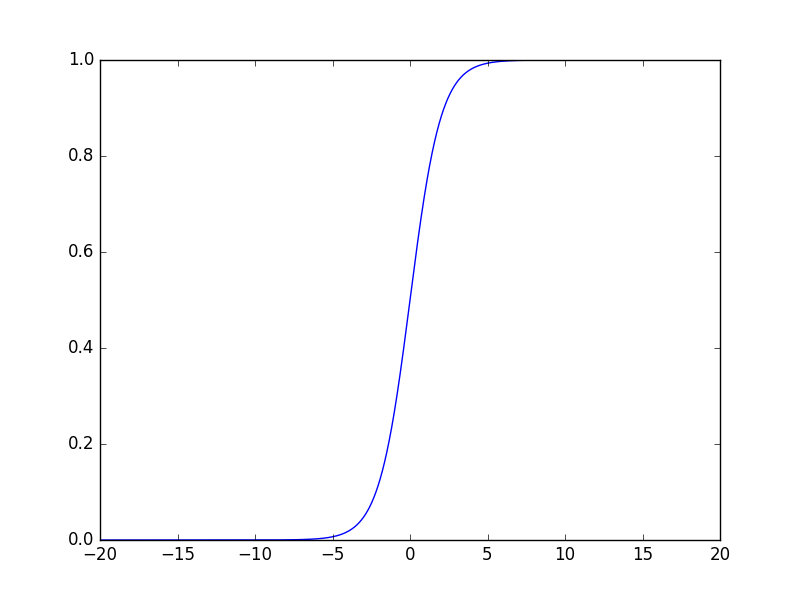
\includegraphics[scale=0.5]{images/sigmoid_graph.png}
\caption{Graf sigmoidalne aktivacijske funkcije}
\label{img:sigmoid_graph}
\end{figure}

\noindent Sigmoidalna aktivacijska funkcija preslikava ulaznu vrijednost na vrijednost iz intervala $\left< 0, 1\right>$. Sigmoidalna aktivacijska funkcija je derivabilna na cijeloj domeni i njenim korištenjem dobivamo nelinearne modele. 
Slika \ref{img:sigmoid_graph} prikazuje graf sigmoidalne aktivacijske funkcije. 
Iz njega je vidljivo kako će gradijent za većinu vrijednosti sigmoidalne funkcije biti vrlo niska zbog toga što je vrijednost sigmoidalne funkcije gotovo na cijeloj domeni u zasićenju \engl{saturating function} — asimptotski se približava vrijednosti 0 ili 1.
Kako je ranije navedeno, učenje modela obavljamo koristeći gradijentni spust funkcije gubitka po parametrima modela. 
Uglavnom nizak iznos gradijenta utječe na to da će već u zadnjem, izlaznom sloju korekcije parametara mreže biti vrlo male. 
Kako izračun korekcija propagiramo unatrag, slojevi koji su sve dalje od završnog sloja imat će sve manje iznose korekcija što će uvelike utjecati na brzinu i kvalitetu učenja koje će se drastično smanjiti.
Sigmoidalne aktivacijske funkcije se u praksi zato ne koriste u dubokim modelima \citep{seminar:rela}.

\subsubsection{Po dijelovima linearna aktivacijska funkcija}
Po dijelovima linearna aktivacijska funkcija, ReLU \engl{Rectified Linear Unit} i njena derivacija definirane su kao:
\begin{align}
 g^{(i)}_j(\mathbf{x})&=\left\{
 \begin{array}{ll}
 0,  & \mbox{ako je } x_j < 0 \\
 x_j, & \mbox{ako je } x_j \geq 0 
 \end{array}
 \right. , \\
 \frac{dg^{(i)}_j(\mathbf{x})}{d\mathbf{x}}&=\left\{
 \begin{array}{ll}
 0,  & \mbox{ako je } x_j < 0 \\
 1, & \mbox{ako je } x_j \geq 0 
 \end{array}
 \right.
\end{align}

\begin{figure}[H]
\centering
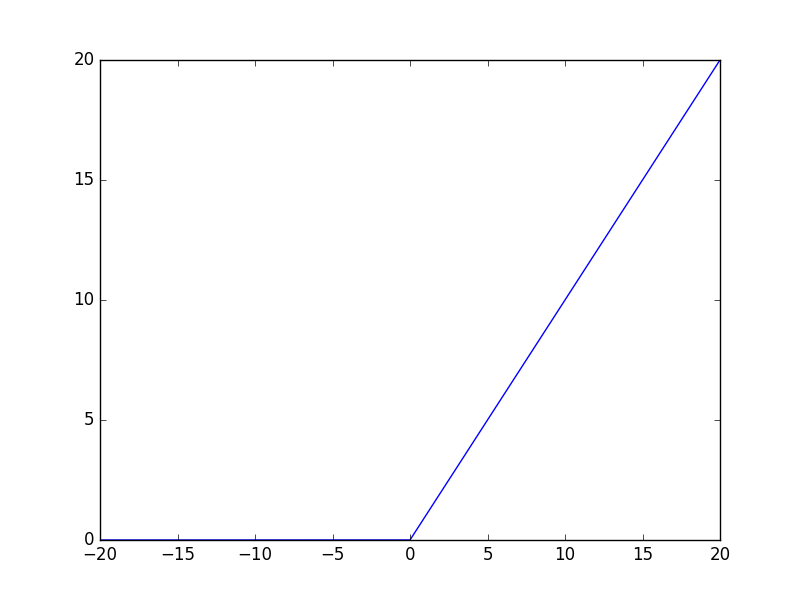
\includegraphics[scale=0.5]{images/relu_graph.png}
\caption{Graf po dijelovima linearne aktivacijske funkcija}
\label{img:relu_graph}
\end{figure}

\noindent Po dijelovima linearna aktivacijska funkcija predstavlja funkciju praga na vrijednosti $0$ ispod koje izlazne vrijednosti nisu propuštene.
Po dijelovima linearna aktivacijska funkcija je često korištena u dubokim modelima zbog zanimljivih svojstava koja pokazuje prilikom učenja takvih struktura.
Vrijednost gradijenta je kod po dijelovima linearne aktivacijske funkcije konstantna za polovicu cijele njene domene. 
U drugoj polovici iznosi $0$, što ponekad također može biti problem jer može dovesti do mrtvih dijelova slojeva kojima se parametri nikako ne korigiraju.
Problem mrtvih dijelova slojeva može se riješiti korištenjem tzv. leaky ReLU prijenosne funkcije koja dozvoljava mali iznos gradijenta kada je vrijednost aktivacije $0$ \citep{book:deeplearningbook} \citep{seminar:rela}.

\subsubsection{Normalizirajuća eksponencijalna aktivacijska funkcija}
Normalizirajuća eksponencijalna aktivacijska funkcija \engl{softmax} i njena derivacija definirane su kao:
\begin{align}
 g^{(i)}_j(\mathbf{x})&=\cfrac{e^{x_j}}{\sum_{k=1}^{n} e^{x_k}}, \\
 \frac{dg^{(i)}_j(\mathbf{x})}{\mathbf{x}}&=\left\{
 \begin{array}{ll}
 g^{(i)}_j(\mathbf{x}) (1-g^{(i)}_j(\mathbf{x})),  & \mbox{ako je } j = k \\
 -g^{(i)}_j(\mathbf{x}) g^{(i)}_k(\mathbf{x}), & \mbox{ako je } j \neq k 
 \end{array}
 \right.
\end{align}
Normalizirajuća eksponencijalna aktivacijska funkcija je generalizacija sigmoidalne funkcije u smislu da proširuje sigmoidalnu funkciju namijenjenu binarnoj klasifikaciji na klasifikaciju s $n$ klasa.

Normalizirajuća eksponencijalna aktivacijska funkcija preslikava $n$ - dimenzionalni vektor realnih vrijednosti u $n$ - dimenzionalni vektor realnih vrijednosti koje se zbrajaju u vrijednost $1$.
Takav vektor realnih vrijednosti možemo promatrati kao vjerojatnosnu razdiobu i upravo iz tog razloga se normalizirajuća eksponencijalna aktivacijska funkcija često koristi u posljednjem sloju dubokih modela za probleme klasifikacije -- daje nam vjerojatnost s kojom ulazni uzorak pripada svakoj od $n$ mogućih klasa, slično kao što je sigmoidalna aktivacijska funkcija korištena kod binarne klasifikacije logističkom regresijom \citep{seminar:rela}.

\subsection{Konvolucijski sloj}
Konvolucijski slojevi koriste se za stvaranje mapa značajki uporabom dvodimenzionalne konvolucije jezgre s podacima.
Za definiciju konvolucije potrebno je prvo definirati veličinu jezgre (širinu i visinu), vrijednosti parametara jezgre te pomak jezgre po širini odnosno po visini prilikom izračuna.
\begin{figure}[H]
\centering
\includegraphics[scale=0.4]{images/convolution.png}
\caption{Dva koraka konvolucije s dvodimenzionalnim podacima}
\label{img:convolution}
\end{figure}
Slika \ref{img:convolution} prikazuje dva koraka konvolucije podataka s jezgrom. Slika a) prikazuje prvi korak konvolucije, a slika b) drugi korak. 
U oba koraka veličina jezgre je $3x3$, a korak iznosi $1$. 
Korak konvolucije \engl{stride} određuje pomak prozora po širini, odnosno visini ulazne mape značajki. 

Općenito, vrijednost jednog elementa mape značajki u sloju $l$ dobivene konvolucijom nad jednom ulaznom mapom značajki iz sloja $l-1$ definiramo kao:
\begin{equation}
 x^l_{i,j}=\sum_{m,n=0}^{m=K_w,n=K_h}x^{l-1}_{i \cdot s_w +m, j \cdot s_h +n} w^l_{m, n}, \label{eq:convolution}
\end{equation}
gdje je $x_{i,j}^l$ vrijednost mape značajki u sloju $l$, za redak $i$ i stupac $j$. $K_w$ je širina jezgre, $K_h$ je visina jezgre, a $w^l_{m,n}$ vrijednost parametara jezgre za redak $m$ i stupac $n$.
Vrijednosti $s_w$ i $s_h$ predstavljaju pomak po širini, odnosno visini.

Izraz \ref{eq:convolution} opisuje izračun vrijednosti jednog elementa mape značajke koji je linearna kombinacija vrijednosti samo jedne mape značajki prethodnog sloja.
U konvolucijskim arhitekturama se općenito koriste mape značajki koje su povezane s većim brojem mapa značajki iz prethodnog sloja.
Za svaku od mapa značajki s kojom je povezana postoji po jedna jezgra koja se koristi za izračun vrijednosti.
Primjerice, jedna mapa značajki ulaznog sloja može biti povezana s 3 mapa značajki - crvenom, plavom i zelenom komponentom slike u boji.
Za svaku od komponenti boja će mapa značajki tada imati drukčiju jezgru.

Nadalje, izračun vrijednosti mapa značajki se često generalizira kao i kod potpuno povezanog sloja pa se dodaje dodatan parametar kao vrijednost praga te se koriste aktivacijske funkcije.
Generalizirani izraz za izračun vrijednosti jednog elementa mape značajki u sloju $n$ dobivene konvolucijom odgovarajućih jezgri sa svakom od mapa značajki iz sloja $n-1$ s kojima je povezana definiramo kao:
\begin{equation}
 x^l_{k',i,j}=\sigma\left(\sum_{k\in F^{l-1}}\sum_{m,n=0}^{m=K_w^k,n=K_h^k}x^{l-1}_{k, i \cdot s_w +m, j \cdot s_h +n} w^l_{k, m, n} + b^l\right), \label{eq:generalized_convolution}
\end{equation}
gdje je $x_{k,i,j}^l$ vrijednost mape značajki $k$ u sloju $l$, za redak $i$ i stupac $j$. 
$F^{l-1}$ je skup mapa značajki iz sloja $l-1$ s kojima je mapa značajki iz sloja $l$ povezana. 
$K_w^k$ je širina jezgre, a $K_h^k$ je visina jezgre za mapu značajki $k$ iz sloja $l-1$. 
$w^l_{k, m, n}$ je vrijednost parametara jezgre za mapu značajki $k$ iz sloja $l-1$ za redak $m$ i stupac $n$.
Vrijednosti $s_w$ i $s_h$ predstavljaju pomak po širini, odnosno visini.
Vrijednost $b^l$ predstavlja vrijednost praga za mapu značajku iz sloja $l$. 
U pravilu se vrijednost praga dijeli za cijelu mapu značajki, no to nije nužno te je moguće za svaku od mapa značajki iz prethodnog sloja imati po jednu vrijednost praga.
Konačno, funkcija $\sigma$ predstavlja aktivacijsku funkciju.

Zbog svojih svojstava, konvolucijski slojevi mogu uvelike poboljšati učinkovitost modela za klasifikaciju slika.
Konvolucijski slojevi su tipično rijetko povezani --- nije nužno da su sve mape značajki sloja $l-1$ povezane sa svakom od mapa značajki iz sloja $l$ \citep{book:deeplearningbook}, što uz jezgre koje su tipično mnogo manjih veličina od ulaza nad kojima djeluju u velikoj mjeri smanjuje broj parametara i povećava efikasnost učenja i računanja.
Potpuno povezani slojevi koriste matrično množenje i svaki parametar je iskorišten samo jednom za opisivanje veze između ulaza i izlaza, dok se konvolucijom isti parametri koriste za više lokacija ulaza i predstavljaju svojevrsne značajke koje jezgra izlučuje na slici.
Konvolucijske arhitekture korištenjem jezgara s dijeljenim parametrima uče skup parametara koji je otporan na translacije jer će za iste ulazne vrijednosti jezgra dati iste izlazne vrijednosti, bez obzira gdje na slici se one pojave. 
Naučeni dijeljeni skup parametara predstavlja jednu funkciju koju jezgra obavlja (primjerice, detekcija rubova) -- učenjem se skup parametara prilagođava cijeloj slici i uči se tako da obavlja apstraktne funkcije neovisne o lokaciji slike, a koje će pripomoći u samoj klasifikaciji.
Nabrojana svojstva konvolucijske arhitekture donose svojevrsnu ugrađenu regularizaciju što povlači bolju generalizaciju uz veću efikasnost \citep{book:deeplearningbook} \citep{masters:vukotic_ms} \citep{seminar:rela}.

\subsection{Sloj sažimanja}
Slojevi sažimanja koriste se da se grupira određeni broj podataka mape značajki i predstavi ih kao jedan podatak koji statistički dobro predstavlja tu grupu.
Sam postupak također smanjuje veličinu mapa značajki i to tako da ih skalira faktorom $\cfrac{1}{S_w}$ po širini, odnosno faktorom $\cfrac{1}{S_h}$ po visini, gdje je $S_w$ širina, a $S_h$ visina podmape značajki koja se grupira.

Korisnost postupka očituje se u vidu ostvarivanja invarijantnosti na lokalne translacije što može biti vrlo korisno u slučaju da nam je bitnije da je neka značajka prisutna od toga na kojoj je točno lokaciji \citep{seminar:rela}.

Postoje različite vrste funkcija koje se koriste za sažimanje od kojih je u ovom radu korištena sljedeća:
\begin{description}  
\item [sažimanje maksimalnom vrijednošću]
Sažimanje maksimalnom vrijednošću \engl{max-pooling} grupira značajke tako da iz podmape značajki nad kojom djeluje izluči samo maksimalnu vrijednost koja postaje predstavnik.
Sažimanje maksimalnom vrijednošću je najpopularnija metoda sažimanja i pokazuje se da ima vrlo dobre rezultate i performanse \citep{article:maxpooling_article}.
\end{description}

\subsection{Sloj grupne normalizacije \engl{batch normalization}}
Učenje dubokih modela može biti vrlo komplicirano ukoliko bolje promotrimo njihovu arhitekturu, način učenja i sam utjecaj načina učenja na brzinu učenja.
Učenjem mijenjamo parametre modela, a samim time, promjenom parametara u određenom sloju modela, mijenjamo distribuciju ulaznih podataka koje dobiva idući sloj.
Sama dubina dodatno uvećava utjecaj promjena parametara modela -- distribucija ulaza svakog sloja uvjetovana je promjenama na parametre modela svih slojeva koji mu prethode.

Konstantna promjena distribucije ulaza slojeva predstavlja problem jer je potrebno stalno se prilagođavati na novu distribuciju, što može uvelike usporiti učenje.
Opisani problem nazivamo interni kovarijacijski pomak \engl{internal covariate shift}. 
Metoda grupne normalizacije \engl{Batch Normalization} uklanja taj problem i uvelike ubrzava učenje dubokih modela.

Uklanjanje problema internog kovarijacijskog pomaka rješavamo normalizacijom ulaza svakog sloja -- linearno ga transformiramo tako da mu je srednja vrijednost jednaka 0, a varijanca mu je jednaka 1.
Direktna normalizacija ulaza i izlaza nekog sloja ovisi o statistici svih ulaza tog sloja nad kompletnim skupom podataka nad kojim učimo mrežu.
Zbog izrazite računske složenosti koja bi bila potrebna za to, uvode se neka pojednostavljenja.

Prva pretpostavka za pojednostavljenje složenosti jest da umjesto normalizacije ulaza i izlaza združeno, normaliziramo svaku komponentu ulaza zasebno, s pretpostavkom da komponente nisu međusobno zavisne.
Normalizacija $k$-te komponente ulaznog vektora $\mathbf{x}$ nekog sloja definirana je na sljedeći način:
\begin{equation}
 \hat{\mathbf{x}}^{(k)} = \cfrac{\mathbf{x}^{(k)} - \mathop{\mathbb{E}} \left[ \mathbf{x}^{(k)} \right]} {\sqrt{ \mathrm{Var} \left[ \mathbf{x}^{(k)} \right] } }, \label{eq:bn_normalization}
\end{equation}
gdje su očekivanje i varijanca izračunati nad skupom podataka za učenje.
Normalizacija svakog ulaza nekog sloja može promijeniti njegovu ekspresivnu snagu pa iz tog razloga uvodimo transformaciju normaliziranog ulaza kojom osiguravamo da je iz normaliziranih ulaznih podataka moguće dobiti originalne vrijednosti.
Transformacija $k$-te komponente prethodno normaliziranog ulaznog vektora $\hat{\mathbf{x}}$ nekog sloja definirana je na sljedeći način:
\begin{equation}
 \mathbf{y}^{(k)} = \boldsymbol{\gamma}^{(k)} \hat{\mathbf{x}}^{(k)} + \boldsymbol{\beta}^{(k)}, \label{eq:bn_transformation}
\end{equation}
gdje su $\boldsymbol{\gamma}^{(k)}$ i $\boldsymbol{\beta}^{(k)}$ parametri koji se uče zajedno s parametrima modela i koji omogućuju skaliranje i pomak normalizirane vrijednosti izlaza.

Druga pretpostavka za pojednostavljenje složenosti jest da normalizaciju umjesto nad statistikom cjelokupnog skupa podataka za učenje, obavljamo nad statistikama malih podskupova podataka \engl{mini-batch}.
Grupna normalizacija nad statistikom malog podskupa skupa podataka za učenje u nekom sloju tada je definirana kao normalizacija i linearna transformacija ulaza, definirane u izrazima \ref{eq:bn_normalization} i \ref{eq:bn_transformation}.

Transformacija grupne normalizacije najčešće se koristi nad izračunatim težinskim sumama slojeva, prije djelovanja aktivacijske funkcije.
Normalizirane vrijednosti $\hat{\mathbf{x}}^{(k)}$ možemo promatrati kao ulaze u podsloj kojem je funkcija linearna, i to je upravo funkcija transformacije definirana u izrazu \ref{eq:bn_transformation}.
Na izlaz podsloja tada djeluje procesiranje originalnog sloja. 
Takvom arhitekturom ostvarili smo da svi podslojevi na ulaze dobivaju podatke s fiksnom distribucijom (s očekivanjem 0 i varijancom 1), što ubrzava učenje podslojeva, a time posljedično i samih slojeva i kompletne mreže \citep{article:bn_paper} \citep{seminar:rela}.

\section{Arhitekture korištene u eksperimentima}
U poglavlju \ref{chapter:skupovi_podataka} opisana su dva tipa skupova podataka korištenih za eksperimente -- skup podataka sa statičnim slikama i skup podataka sa sekvencama slika.
Korišteno je nekoliko različitih modela koji su zasnovani na arhitekturi VGG-16 \citep{article:vgg} treniranoj za natjecanje ILSVRC-2014 \citep{article:ilsvrc2015}.
Model VGG-16 treniran je za klasifikaciju slika u 1000 različitih klasa na vrlo velikom broju slika -- 1.3 milijuna \citep{article:vgg}.
Pokazuje se da model iz tog razloga vrlo dobro generalizira i na drugim problemima \citep{article:vgg} pa je iz tog razloga odabran kao baza modela korištenih za eksperimente u ovom radu.

\subsection{Arhitektura VGG-16 modela}
\begin{figure}[H]
\centering
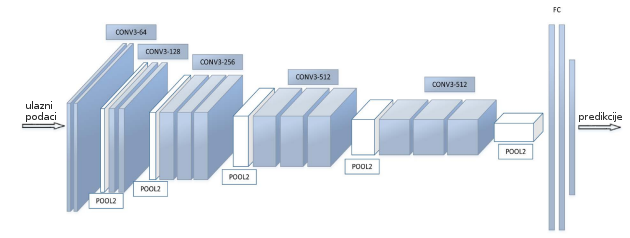
\includegraphics[scale=0.65]{images/vgg_architecture.png}
\caption{Arhitektura VGG-16 modela, preuzeto i prerađeno iz \citep{article:vgg_architecture}}
\label{img:vgg_architecture}
\end{figure}
Slika \ref{img:vgg_architecture} prikazuje originalnu arhitekturu VGG-16 građenu od 16 slojeva.

Prednji dio sastoji se od 5 konvolucijskih blokova. 
Svaki od blokova izgrađen je na sličan način -- nekoliko konvolucijskih slojeva iza kojih slijedi sloj za sažimanje maksimalnom vrijednošću \engl{max pool}.
Konvolucijski slojevi imaju jezgre dimenzija $3$ x $3$ uz korak konvolucije \engl{stride} 1. 
Svi konvolucijski slojevi koriste po dijelovima linearnu funkciju \engl{ReLU} te su regularizirani L2 regularizacijom s faktorom regularizacije iznosa $5\cdot10^{-4}$.
Slojevi za sažimanje maksimalnom vrijednošću imaju podmape za grupiranje veličine $2$ x $2$ uz korak uzorkovanja podmapa 2.
Konvolucijski blokovi građeni su kako slijedi:
\begin{itemize}
 \item prvi konvolucijski blok:
 \begin{itemize}
  \item konvolucijski sloj sa 64 izlaznih mapi značajki
  \item konvolucijski sloj sa 64 izlaznih mapi značajki
  \item sloj za sažimanje maksimalnom vrijednošću
 \end{itemize}
  \item drugi konvolucijski blok:
 \begin{itemize}
  \item konvolucijski sloj sa 128 izlaznih mapi značajki
  \item konvolucijski sloj sa 128 izlaznih mapi značajki
  \item sloj za sažimanje maksimalnom vrijednošću
 \end{itemize}
   \item treći konvolucijski blok:
 \begin{itemize}
  \item konvolucijski sloj s 256 izlaznih mapi značajki
  \item konvolucijski sloj s 256 izlaznih mapi značajki
  \item konvolucijski sloj s 256 izlaznih mapi značajki
  \item sloj za sažimanje maksimalnom vrijednošću
 \end{itemize}
    \item četvrti konvolucijski blok:
 \begin{itemize}
  \item konvolucijski sloj s 512 izlaznih mapi značajki
  \item konvolucijski sloj s 512 izlaznih mapi značajki
  \item konvolucijski sloj s 512 izlaznih mapi značajki
  \item sloj za sažimanje maksimalnom vrijednošću
 \end{itemize}
     \item peti konvolucijski blok:
 \begin{itemize}
  \item konvolucijski sloj s 512 izlaznih mapi značajki
  \item konvolucijski sloj s 512 izlaznih mapi značajki
  \item konvolucijski sloj s 512 izlaznih mapi značajki
  \item sloj za sažimanje maksimalnom vrijednošću
 \end{itemize}
\end{itemize}

Stražnji dio građen je od  3 potpuno povezana sloja koji služe za klasifikaciju slika u 1000 različitih klasa. 
Prilikom korištenja VGG-16 arhitekture obično se uklanja stražnji ili svi potpuno povezani slojevi te se na prednji dio koji služi za izlučivanje značajki iz ulaznih slika nadodaju novi slojevi koji se treniraju za obavljanje specifičnog zadatka.

\subsection{Arhitektura za klasifikaciju pojedinačnih slika}
Duboki model korišten za klasifikaciju pojedinačnih slika temeljen je na VGG-16 arhitekturi. 
Koristi se naučen prednji dio s 5 konvolucijskih blokova. 
Dobivene izlazne mape značajki pretvaraju se u jednodimenzionalan vektor koji se zatim vodi na potpuno povezane slojeve koji su definirani kako slijedi:
\begin{itemize}
 \item potpuno povezani sloj dimenzionalnosti 200
 \begin{itemize}
  \item po dijelovima linearna \engl{ReLU} aktivacijska funkcija
  \item grupna normalizacija \engl{batch normalization}
  \item L2 regularizacija
 \end{itemize}
 \item potpuno povezani sloj dimenzionalnosti 2 za binarnu klasifikaciju -- određivanje je li atribut prisutan na slici ili nije
 \begin{itemize}
  \item normalizirajuća eksponencijalna \engl{softmax} aktivacijska funkcija
  \item L2 regularizacija
 \end{itemize}
\end{itemize}

\subsection{Arhitekture za klasifikaciju sekvenci slika}
Za klasifikaciju sekvenci slika korišteno je nekoliko različitih modela temeljenih na naučenoj VGG-16 arhitekturi. 
Korišteni modeli su inspirirani arhitekturama iz \citep{article:sequential_architectures}.

Zajednički postupak koji svi modeli dijele jest postupak izlučivanja prostornih značajki -- za svaku sliku sekvence se koristeći prednji dio naučenog VGG-16 modela izračunaju značajke koje se zatim dalje obrađuju na različite načine.
Dobivene prostorne značajke svake pojedine slike su dimenzija $H$ x $W$ x $512$, gdje dimenzije $H$ i $W$ ovise o dimenzijama ulaznih slika, a treća dimenzija je određena brojem izlaznih mapi značajki posljednjeg konvolucijskog sloja VGG-16 modela. 

\subsubsection{Klasifikacija sekvenci slika korištenjem vremensko-prostornog sažimanja}
Model koji koristi vremensko-prostorno sažimanje prostorne značajke svake slike pretvori u jednodimenzionalni vektor dimenzija $H$ x $W$ x $512$.
Dobiveni jednodimenzionalni vektori se zatim oblikuju u dvodimenzionalnu strukturu dimenzija $N$ x ($H$ x $W$ x $512$), gdje je $N$ duljina sekvence slika.

Dvodimenzionalna struktura koja se dobije povezivanjem prostornih značajki sadrži i vremenske i prostorne informacije. 
Dobivena dvodimenzionalna zatim se obrađuje kroz nekoliko slojeva kako slijedi:
\begin{itemize}
 \item sloj za sažimanje maksimalnom vrijednošću s podmapama za grupiranje veličina $2$ x $2$ uz korak uzorkovanja podmapa 2
 \begin{itemize}
  \item operacija efektivno provodi vremensko-prostorno sažimanje značajki koje su bliske vremenski i prostorno
 \end{itemize}
 \item pretvaranje dobivene dvodimenzionalne strukture u jednodimenzionalnu
 \item potpuno povezani sloj dimenzionalnosti 200
 \begin{itemize}
  \item po dijelovima linearna \engl{ReLU} aktivacijska funkcija
  \item grupna normalizacija \engl{batch normalization}
  \item L2 regularizacija
 \end{itemize}
 \item potpuno povezani sloj dimenzionalnosti 2 za binarnu klasifikaciju -- određivanje je li atribut prisutan na slici ili nije
 \begin{itemize}
  \item normalizirajuća eksponencijalna \engl{softmax} aktivacijska funkcija
  \item L2 regularizacija
 \end{itemize}
\end{itemize}

\subsubsection{Klasifikacija sekvenci slika korištenjem povratnih LSTM ćelija \engl{Long Short Term Memory}}
\begin{figure}[H]
\centering
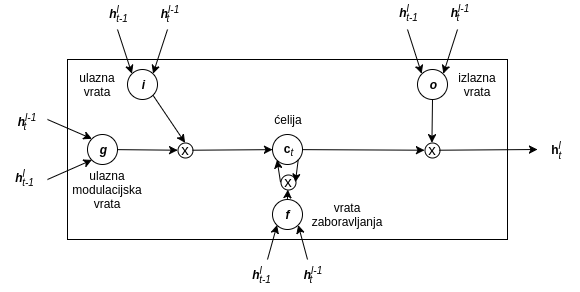
\includegraphics[scale=0.6]{images/lstm.png}
\caption{Arhitektura LSTM ćelije, nacrtano prema \citep{article:lstm}}
\label{img:lstm}
\end{figure}
Slika \ref{img:lstm} prikazuje arhitekturu LSTM ćelije. 
LSTM ćelije pogodne su za korištenje nad sekvencama podataka iz razloga što sadrže memorijske ćelije u kojima mogu čuvati informacije kroz dugačke vremenske periode.

U svakom vremenskom koraku potrebno je izračunati izlaz LSTM ćelije i novi sadržaj memorijske ćelije.
Izlaz LSTM ćelije i novi sadržaj memorijske ćelije računaju se na temelju tri stvari:
\begin{itemize}
 \item izlaz iz LSTM ćelije iz prethodnog sloja za trenutni vremenski korak (ili ulazni podatak trenutnog vremenskog koraka ukoliko je riječ o prvom sloju LSTM ćelija) -- $\mathbf{h}_{l-1}^t$ na slici \ref{img:lstm}
 \item izlaz iz LSTM ćelije trenutnog sloja za prethodni vremenski korak  -- $\mathbf{h}_{l}^{t-1}$ na slici \ref{img:lstm}
 \item sadržaj memorijske ćelije trenutnog sloja za prethodni vremenski korak -- $\mathbf{c}_t$ na slici \ref{img:lstm}
\end{itemize}
Izlaz LSTM ćelije i novi sadržaj memorijske ćelije računaju se sljedećim izrazima:
\begin{align}
 \mathbf{c}_t^l &= \mathbf{f} \odot \mathbf{c}_{t-1}^l + \mathbf{i} \odot \mathbf{g} \\
 \mathbf{h}_t^l &= \mathbf{o} \odot \tanh(\mathbf{c}^l_t) \\
 \mathbf{i} &= \sigma (\mathbf{W}_i [\mathbf{h}_{l}^{t-1}, \mathbf{h}_{l-1}^t] + \mathbf{b}_i) \\
 \mathbf{f} &= \sigma (\mathbf{W}_f [\mathbf{h}_{l}^{t-1}, \mathbf{h}_{l-1}^t] + \mathbf{b}_f) \\
 \mathbf{o} &= \sigma (\mathbf{W}_o [\mathbf{h}_{l}^{t-1}, \mathbf{h}_{l-1}^t] + \mathbf{b}_o) \\
 \mathbf{g} &= \sigma (\mathbf{W}_g [\mathbf{h}_{l}^{t-1}, \mathbf{h}_{l-1}^t] + \mathbf{b}_g), 
\end{align}
gdje je $\tanh$ aktivacijska funkcija tangens hiperbolni, $\sigma$ je sigmoidalna aktivacijska funkcija, $\odot$ je operator množenja koji djeluje po elementima, a $[\mathbf{x}, \mathbf{y}]$ je operacija spajanja vektora $\mathbf{x}$ dimenzija $n_1$ i vektora $\mathbf{y}$ dimenzija $n_2$ u vektor dimenzija $n_1 + n_2$.

Model koji koristi LSTM ćelije prostorne značajke svake slike pretvori u jednodimenzionalni vektor dimenzija $H$ x $W$ x $512$.
Dobiveni jednodimenzionalni vektori se zatim redom obrađuju kako slijedi:
\begin{itemize}
 \item LSTM sloj sa stanjem dimenzionalnosti 128
 \item LSTM sloj sa stanjem dimenzionalnosti 64
 \item LSTM sloj sa stanjem dimenzionalnosti 32
  \item potpuno povezani sloj dimenzionalnosti 2 za binarnu klasifikaciju -- određivanje je li atribut prisutan na slici ili nije
 \begin{itemize}
  \item ulaz u ovaj potpuno povezani sloj jest posljednji izlaz dobiven iz LSTM ćelije prethodnog sloja koja je obradila cijelu sekvencu podataka (vektor dimenzionalnosti 32)
  \item normalizirajuća eksponencijalna \engl{softmax} aktivacijska funkcija
  \item L2 regularizacija
 \end{itemize}
\end{itemize}


\subsubsection{Klasifikacija sekvenci slika korištenjem vremenskog potpuno povezanog sloja}
Model koji koristi vremenski potpuno povezani sloj prostorne značajke pretvori u jednodimenzionalni vektor dimenzija $H$ x $W$ x $512$.
Svaki dobiveni jednodimenzionalni vektor prostornih značajki se zatim obrađuje kako slijedi:
\begin{itemize}
  \item potpuno povezani sloj dimenzionalnosti 64
 \begin{itemize}
  \item po dijelovima linearna \engl{ReLU} aktivacijska funkcija
  \item grupna normalizacija \engl{batch normalization}
  \item L2 regularizacija
  \item ovaj potpuno povezani sloj služi za predstavljanje prostornih značajki vektorom manjih dimenzija
 \end{itemize}
\end{itemize}
Jednodimenzionalni vektori dobiveni nakon potpuno povezanog sloja se zatim oblikuju u dvodimenzionalnu strukturu dimenzija $N$ x ($H$ x $W$ x $512$), gdje je $N$ duljina sekvence slika.
Dobivena dvodimenzionalna zatim se obrađuje kroz nekoliko slojeva kako slijedi:
\begin{itemize}
 \item pretvaranje dobivene dvodimenzionalne strukture u jednodimenzionalnu
 \item potpuno povezani sloj dimenzionalnosti 64
 \begin{itemize}
  \item po dijelovima linearna \engl{ReLU} aktivacijska funkcija
  \item grupna normalizacija \engl{batch normalization}
  \item L2 regularizacija
  \item ovaj potpuno povezani sloj služi za povezivanje dobivenih prostornih značajki po dimenziji vremena
 \end{itemize}
 \item potpuno povezani sloj dimenzionalnosti 2 za binarnu klasifikaciju -- određivanje je li atribut prisutan na slici ili nije
 \begin{itemize}
  \item normalizirajuća eksponencijalna \engl{softmax} aktivacijska funkcija
  \item L2 regularizacija
 \end{itemize}
\end{itemize}

\section{Postupak pripreme skupova podataka}
Poglavlje \ref{chapter:skupovi_podataka} opisuje dva tipa skupova podataka korištenih u ovom radu.
U nastavku je opisan postupak pretprocesiranja slika dobivenih iz videa sa stranice \citep{url:ftts_irap} te postupak kreiranja slika označenih konzistentno s projektom FTTS iRAP.

\subsection{Pretprocesiranje slika}
Slike korištene za kreiranje skupova podataka dobivene su iz video snimaka snimljenih automobilom koji se kretao engleskim autocestama.
Zbog kretnje automobila uzorkovane slike bit će snimljene iz različitog kuta u odnosu na Sunce.
Takva situacija za posljedicu ima da su neke slike mnogo svjetlije, a neke mnogo tamnije od drugih.

Metoda kojom se može ublažiti velika varijacija kontrasta između slika jest metoda adaptivnog izjednačavanja histograma \citep{article:adapt_hist}.
Izjednačavanje histograma za cilj ima izjednačiti razdiobu intenziteta svih kanala slike (crvenog, zelenog i plavog) na način da oni budu uniformno distribuirani.
Metoda adaptivnog izjednačavanja histograma za računanje histograma ne uzima u obzir cijelu sliku nego prozore određene veličine čime se dobiva na lokalnosti izjednačavanja.

\begin{figure}[H]
\centering
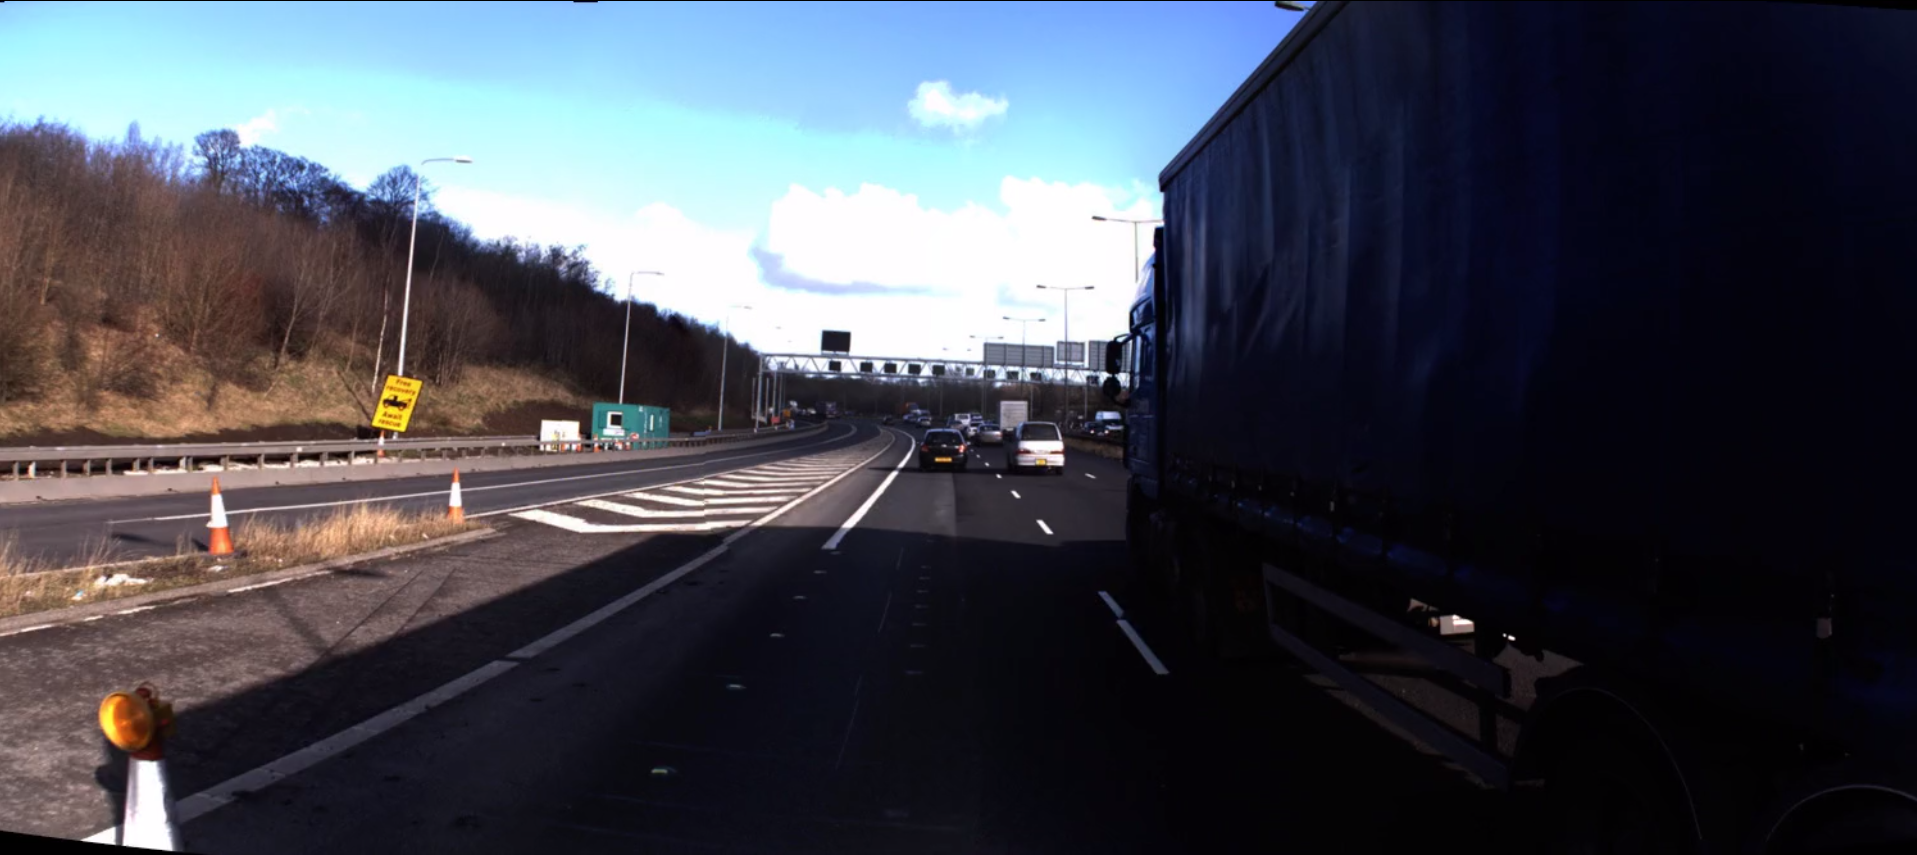
\includegraphics[scale=0.2]{images/original.png}
\caption{Originalna slika, preuzeto s \citep{url:ftts_irap}}
\label{img:original}
\end{figure}

\begin{figure}[H]
\centering
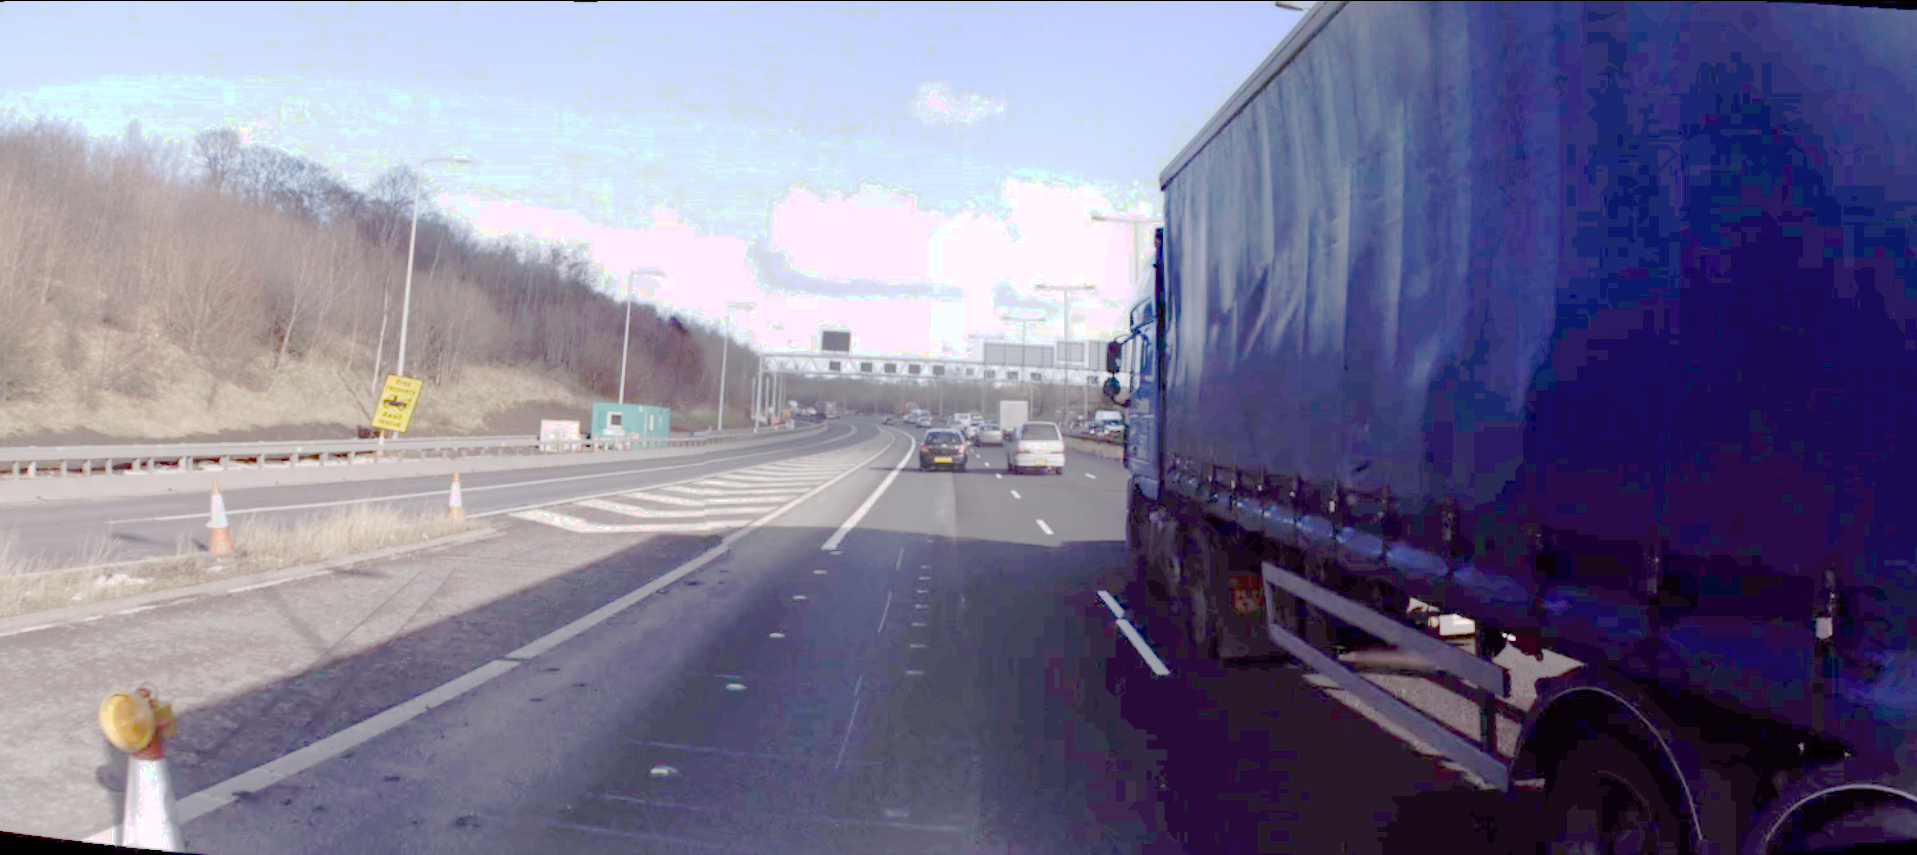
\includegraphics[scale=0.2]{images/hist.png}
\caption{Slika s izjednačenim histogramom, preuzeto s \citep{url:ftts_irap}}
\label{img:hist}
\end{figure}

\begin{figure}[H]
\centering
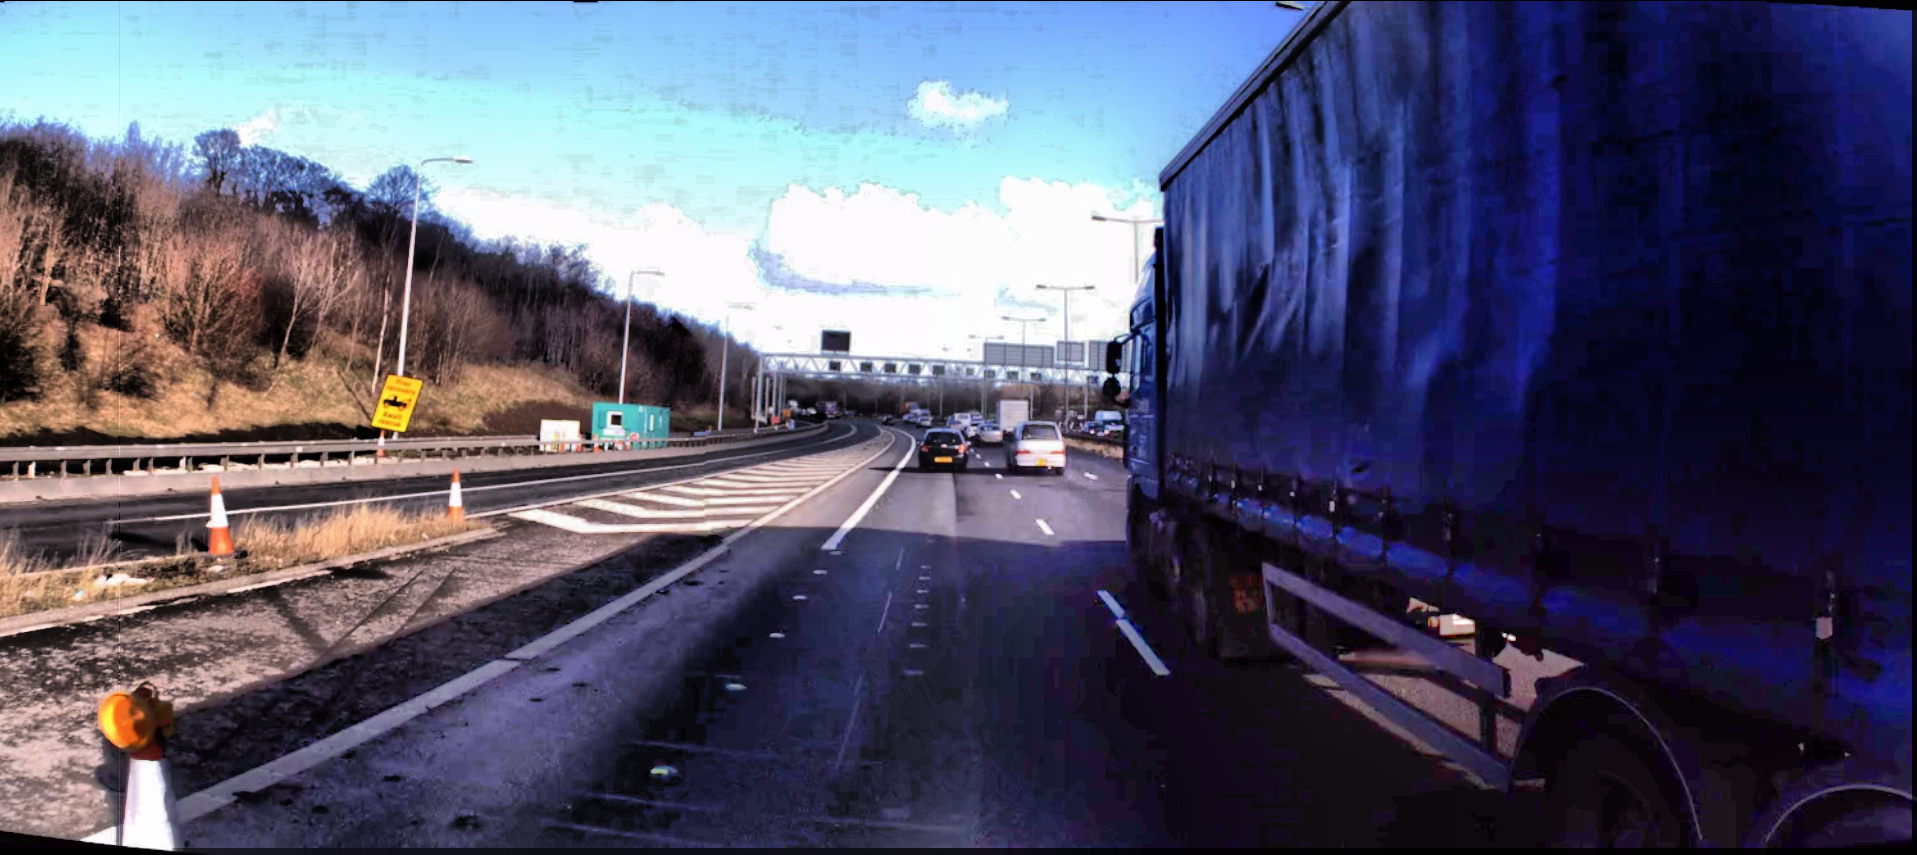
\includegraphics[scale=0.2]{images/adapt_hist.png}
\caption{Slika s adaptivno izjednačenim histogramom, preuzeto s \citep{url:ftts_irap}}
\label{img:adapt_hist}
\end{figure}

Iz slika \ref{img:original}, \ref{img:hist} i \ref{img:adapt_hist} vidljivo je kako su, u odnosu na originalnu sliku, na slici s adaptivno izjednačenim histogramom najbolje naglašeni detalji zbog najbolje ublažene varijacije kontrasta.
Metoda adaptivnog izjednačavanja histograma se iz tog razloga koristi kao korak pretprocesiranja za svaku sliku korištenu prilikom kreiranja skupova podataka.

\subsection{Postupak kreiranja slika označenih konzistentno s projektom FTTS iRAP}
Za postupak kreiranja slika prometnih scena označenih konzistentno s projektom FTTS iRAP kreiran je automatizirani postupak.
Ulazni podaci za automatizirani postupak su sljedeći:
\begin{itemize}
 \item geolokacije na kojima je prisutan atribut pripajanja
 \item popis poveznica na sve video snimke u sustavu \citep{url:ftts_irap}
 \item broj video snimaka koji će se obraditi
\end{itemize}
Postupak će iz ulaznih podataka kreirati sljedeće:
\begin{itemize}
 \item slika s oznakom prisutnosti atributa pripajanja na njoj te sekvenca slika koja joj prethodi (kao što je objašnjeno u poglavlju \ref{chapter:skupovi_podataka})
 \item slika s oznakom prisutnosti atributa pripajanja bez sekvence koja joj prethodi
 \item geolokacije označenih slika i sekvenci slika
\end{itemize}
\noindent Postupak kreira označene slike sa i bez sekvence koja joj prethodi kako bi se eksperimentima ustanovilo dobiva li se na točnosti postupka uvodeći više informacija kroz sekvencu slika.

Geolokacije video sekvence uzorkovane su rijetko -- najčešće svakih $0.5s$. 
Iz tog razloga se za točnu geolokaciju konkretne sličice video sekvence vrši linearna interpolacija između dvije uzorkovane geolokacije koje su vremenski najbliže konkretnoj sličici.
Geolokacija konkretnih sličica korisna je informacija iz razloga što je prilikom testiranja modela za svaki ulazni podatak kojem model dodijeli krivu oznaku moguće u sustavu FTTS iRAP provjeriti je li osoba koja je dodijelila vrijednost atributa tom segmentu to napravila točno ili je riječ o mogućoj pogrešci. 
Takvim postupkom moguće je na brži način validirati ispravnost dodijeljenih oznaka u sustavu.

Nastavak opisuje sažeti pseudokod automatiziranog postupka:
\begin{algorithm}[H]
\caption{Automatizirano kreiranje slika označenih konzistentno s projektom FTTS iRAP}
\label{alg:dataset_creator}
\begin{algorithmic}
\WHILE{nije obrađen željen broj video sekvenci}
\STATE v=preuzmi\_video()
\STATE geolok,vrem=preuzmi\_geolokacije\_i\_vremena(v)
\STATE sl=kreiraj\_sličice(v)
\STATE ind\_geolok,brz\_aut=indeksiraj\_geolokacije\_i\_izračunaj\_brzine\_automobila(geolok,vrem)
\STATE ras\_poz=izračunaj\_raspone\_pozitiva(geolok\_pripajanja,ind\_geolok,brz\_aut)
\STATE poz\_slič,geolok\_slič=kreiraj\_pozitivne\_sličice\_s\_geolokacijama(ras\_poz,sl)
\STATE pohrani\_sličice(poz\_slič,geolok\_slič)
\STATE neg\_slič,geolok\_slič=kreiraj\_negativne\_sličice\_s\_geolokacijama(ras\_poz,sl)
\STATE pohrani\_sličice(neg\_slič,geolok\_slič)
\ENDWHILE
\end{algorithmic}
\end{algorithm}

\noindent Izračunavanje raspona sličica na kojima je prisutan atribut pripajanja (pozitivne sličice) radi se na sljedeći način:
\begin{itemize}
 \item za svako pripajanje i njegovu geolokaciju pronađu se dvije najbliže geolokacije video sekvence
 \item ukoliko je bliža geolokacija video sekvence unutar praga udaljenosti pripajanju, uzima se da je pripajanje prisutno na tom dijelu video sekvence
 \item na temelju udaljenosti geolokacija video sekvence od geolokacije pripajanja i brzina kretanja automobila izračuna se točan raspon vremena video sekvence na kojem se nalazi segment atributa pripajanja
 \item iz dobivenog raspona vremena izračuna se raspon sličica video sekvence na kojem se nalazi segment atributa pripajanja
\end{itemize}

\chapter{Eksperimenti i rezultati}
Za potrebe ovog rada provedeno je nekoliko eksperimenata. 
Postupak učenja i testiranja u svakom eksperimentu je jednak, razlikuju se samo u vrsti ulaznih podataka (statične slike ili sekvence slika) te u korištenoj arhitekturi.

\section{Način učenja i testiranja u eksperimentima}
Početni korak prilikom učenja jest normalizacija skupa podataka.
Kako su podaci slike u boji, na podacima za treniranje se izračunava srednja vrijednost intenziteta piksela za svaki od kanala -- crveni, zeleni i plavi.
Dobivene srednje vrijednosti se zatim po kanalima oduzimaju svim podacima -- podacima za treniranje, podacima za validaciju i podacima za testiranje.

Kako su sve arhitekture korištene za potrebe ovog rada zasnovane na naučenom prednjem dijelu arhitekture VGG-16, učenje se obavlja kroz 50 epoha i to na sljedeći način:
\begin{itemize}
 \item 10 epoha učenja s početnom stopom učenja iznosa $5\cdot10^{-4}$ uz optimiranje samo novo nadodanih parametara -- svi parametri naučenog prednjeg dijela arhitekture VGG-16 ne mijenjaju se tijekom ove faze
 \item 40 epoha učenja s početnom stopom učenja iznosa $1\cdot10^{-5}$ uz optimiranje kompletnog skupa parametara (uključujući i parametre naučenog prednjeg dijela arhitekture VGG-16)
 \item korak učenja koristi gradijente izračunate nad mini-grupama veličina 5 ili 10, ovisno o memorijskoj zahtjevnosti modela
 \item optimizator korišten za učenje jest Adam optimizator
 \item stopa učenja se svakim korakom učenja eksponencijalno smanjuje:
 \begin{align}
  \eta_{t}=\eta_0 \cdot 0.96^{\cfrac{t}{k}},
 \end{align}
gdje je $t$ indeks koraka učenja, a $k$ je broj koraka učenja u jednoj epohi
 \item svi novo nadodani slobodni parametri (isključujući parametre naučenog prednjeg dijela VGG-16 arhitekture) inicijalizirani su na sljedeći način:
 \begin{itemize}
  \item parametri slojeva (isključujući parametre pomaka) s po dijelovima linearnom aktivacijskom funkcijom inicijalizirani su koristeći inicijalizator koji skalira varijancu prema \citep{article:delving_deep_into_rectifiers}
  \item parametri slojeva (isključujući parametre pomaka) s normalizirajućom eksponencijalnom aktivacijskom funkcijom inicijalizirani su koristeći Xavier inicijalizaciju prema \citep{article:delving_deep_into_rectifiers}
  \item parametri pomaka svih slojeva inicijalizirani su s vrijednostima 0
 \end{itemize}

 \item slobodni parametri regularizirani su L2 regularizacijom s faktorom regularizacije iznosa $5\cdot10^{-4}$
 \item podskup za validaciju korišten je za odabir slobodnih parametara modela
 \begin{itemize}
  \item na kraju svake epohe mjeri se performansa modela na podskupu za validaciju
  \item za testiranje se odabire onaj skup parametara koji postiže najbolju performansu na podskupu za validaciju -- ovime se efektivno obavlja regularizacija jer odabiremo onaj skup parametara koji najbolje generalizira
 \end{itemize}
\end{itemize}
Svi eksperimenti provedeni su na nVIDIA grafičkim karticama GTX 1070 i GTX Titan.

Zadatak ovog rada definiran je kao binarna klasifikacija pa možemo iskoristiti 4 definirana tipa predikcija modela: 
\begin{itemize}
 \item TP \engl{true positive} -- slika koja je označena kao pozitivna (atribut pripajanja je prisutan) i za koju je predikcija modela također takva 
 \item TN \engl{true negative} -- slika koja je označena kao negativna (atribut pripajanja nije prisutan) i za koju je predikcija modela također takva
 \item FP \engl{false positive} -- slika koja je označena kao negativna, a predikcija modela je pozitivna
 \item FN \engl{false negative} -- slika koja je označena kao pozitivna, a predikcija modela je negativna
\end{itemize}
Mjere koje su uzimane u obzir prilikom testiranja jesu točnost \engl{accuracy}, preciznost \engl{precision} i odziv \engl{recall}. 
Točnost jest definirana na sljedeći način:
\begin{align}
 \text{točnost} = \cfrac{\text{TP} + \text{TN}}{\text{TP} + \text{TN} + \text{FP} + \text{FN}}
\end{align}
Odziv jest definirana na sljedeći način:
\begin{align}
 \text{odziv} = \cfrac{\text{TP}}{\text{TP} + \text{FN}}
\end{align}
Preciznost jest definirana na sljedeći način:
\begin{align}
 \text{preciznost} = \cfrac{\text{TP}}{\text{TP} + \text{FP}}
\end{align}
Kako je izlaz modela vjerojatnost da je atribut pripajanja prisutan na slici, odnosno da atribut pripajanja nije prisutan na slici, definira se prag kao iznos vjerojatnosti iznad koje se smatra da je atribut prisutan.
Za različite pragove dobivaju se različite vrijednosti preciznosti i odziva modela prilikom evaluacije. 
Ucrtavanjem svih točaka koje povezuju vrijednost preciznosti i odziva za različite pragove dobivamo graf ovisnosti preciznosti i odziva.
Prosječna preciznost jest definirana kao površina ispod tog grafa.

\section{Klasifikacija ručno označenih slika na različitim rezolucijama}
Eksperimenti na ručno označenim slikama provedeni su koristeći arhitekturu za klasifikaciju pojedinačnih slika. 
Kako su eksperimenti nad sekvencama slika memorijski mnogo zahtjevniji od eksperimenata na pojedinačnim slikama, svrha ovog eksperimenta bila je utvrditi
na kojoj rezoluciji ulaznih slika model gubi ekspresivnu moć i ne uspijeva dati zadovoljavajuću performansu.

Za početnu, originalnu rezoluciju pojedinačnih slika odabrana je rezolucija $700$x$280$. Eksperiment je proveden redom na sljedećim rezolucijama:
$700$x$280$, $525$x$210$, $350$x$140$ i $175$x$70$. Rezultati su dani u nastavku.

\subsection{Rezultati na rezoluciji 700x280}
Konačni rezultati dobiveni za eksperiment s ulaznim podacima rezolucije $700$x$280$ su sljedeći:
\begin{table}[H]
\centering
\caption{Statistički rezultati na rezoluciji $700$x$280$}
\label{score:single_hand_700x280}
\begin{tabular}{|c|c|c|c|c|}
\hline
podskup podataka      & točnost & preciznost & odziv & prosječna preciznost \\ \hline
podskup za učenje     & 1.0     & 1.0        & 1.0  & 1.0 \\ \hline
podskup za validaciju & 0.91     & 0.98        & 0.83  & 0.99 \\ \hline
podskup za testiranje & 0.95     & 0.99          & 0.91  & 0.99 \\ \hline
\end{tabular}
\end{table}
\begin{table}[H]
\centering
\caption{Odnos predikcija modela i stvarnih oznaka na rezoluciji $700$x$280$ na podskupu za učenje}
\label{score:single_hand_700x280_tpfptnfn_train}
\begin{tabular}{|c|c|c|}
\hline
\diagbox{stvarna oznaka}{predikcija modela} & 0  & 1  \\ \hline
0                                & 898 & 0 \\ \hline
1                                & 0 & 902 \\ \hline
\end{tabular}
\end{table}
\begin{table}[H]
\centering
\caption{Odnos predikcija modela i stvarnih oznaka na rezoluciji $700$x$280$ na podskupu za validaciju}
\label{score:single_hand_700x280_tpfptnfn_valid}
\begin{tabular}{|c|c|c|}
\hline
\diagbox{stvarna oznaka}{predikcija modela} & 0  & 1  \\ \hline
0                                & 308 & 5 \\ \hline
1                                & 54 & 259 \\ \hline
\end{tabular}
\end{table}
\begin{table}[H]
\centering
\caption{Odnos predikcija modela i stvarnih oznaka na rezoluciji $700$x$280$ na podskupu za testiranje}
\label{score:single_hand_700x280_tpfptnfn_test}
\begin{tabular}{|c|c|c|}
\hline
\diagbox{stvarna oznaka}{predikcija modela} & 0  & 1  \\ \hline
0                                & 295 & 2 \\ \hline
1                                & 26 & 271 \\ \hline
\end{tabular}
\end{table}
\noindent Tablica \ref{score:single_hand_700x280} prikazuje rezultate dobivene evaluacijom modela koji je postigao najbolju performansu na podskupu za validaciju prilikom učenja.
Tablice \ref{score:single_hand_700x280_tpfptnfn_train}, \ref{score:single_hand_700x280_tpfptnfn_valid} i \ref{score:single_hand_700x280_tpfptnfn_test} prikazuju odnos predikcija modela i stvarnih oznaka kroz matricu zabune.

\begin{figure}[H]
\centering
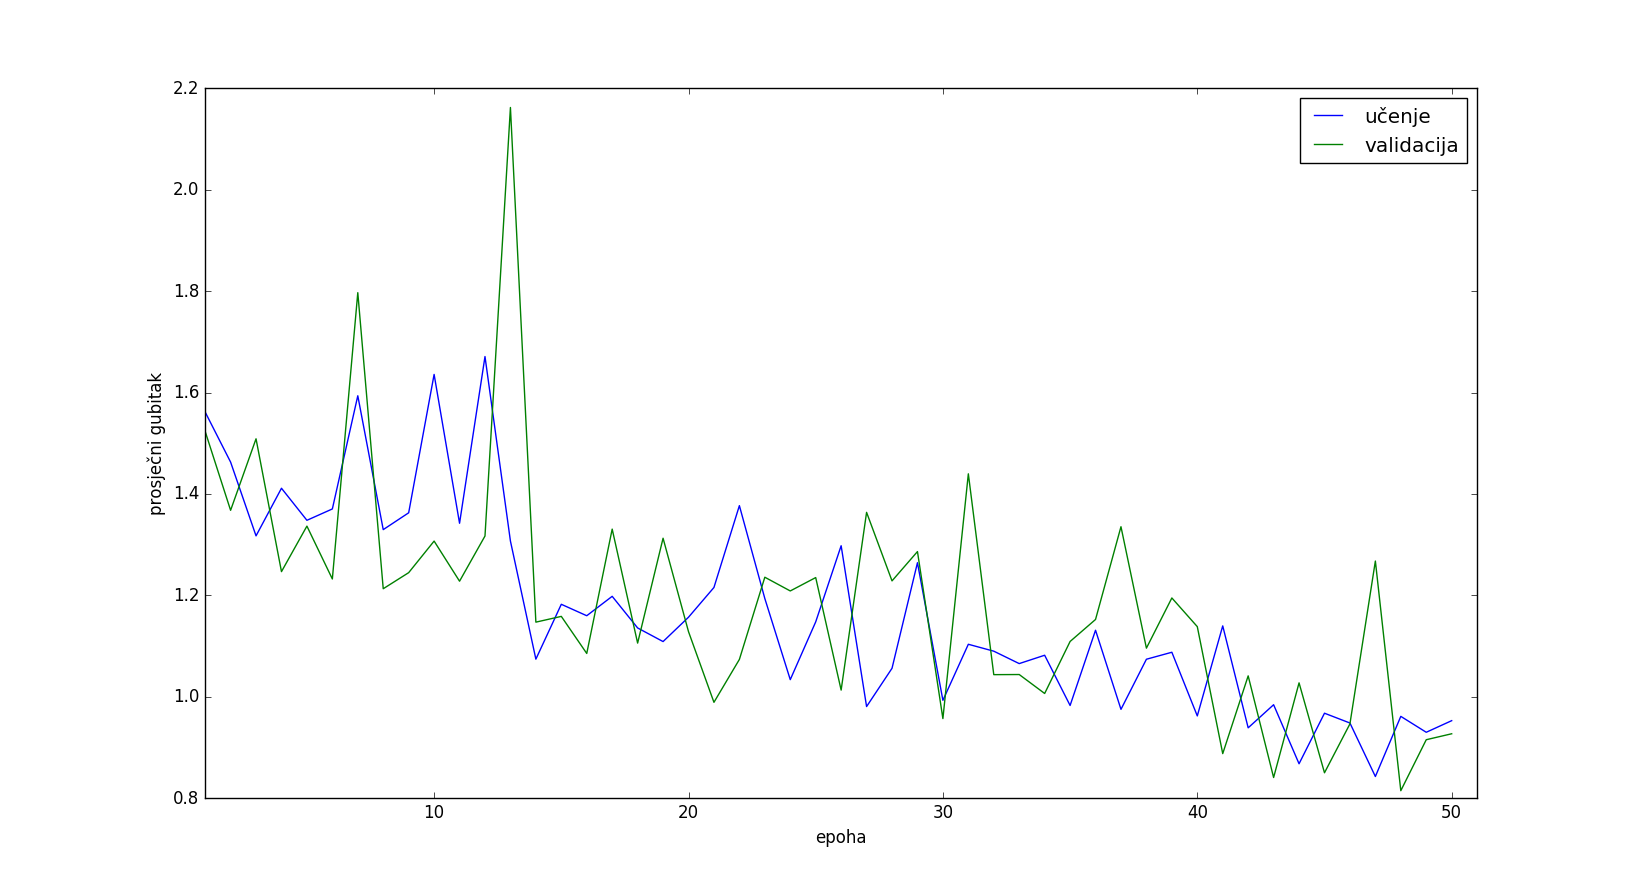
\includegraphics[scale=0.35]{images/single_hand_scale1_loss.png}
\caption{Kretanje prosječnog gubitka na podskupu za učenje i validaciju po epohama}
\label{img:single_hand_scale1_loss}
\end{figure}
\noindent Na slici \ref{img:single_hand_scale1_loss} vidljivo je kretanje prosječnog gubitka po epohama na podskupu za učenje i na podskupu za validaciju.

\begin{figure}[H]
\centering
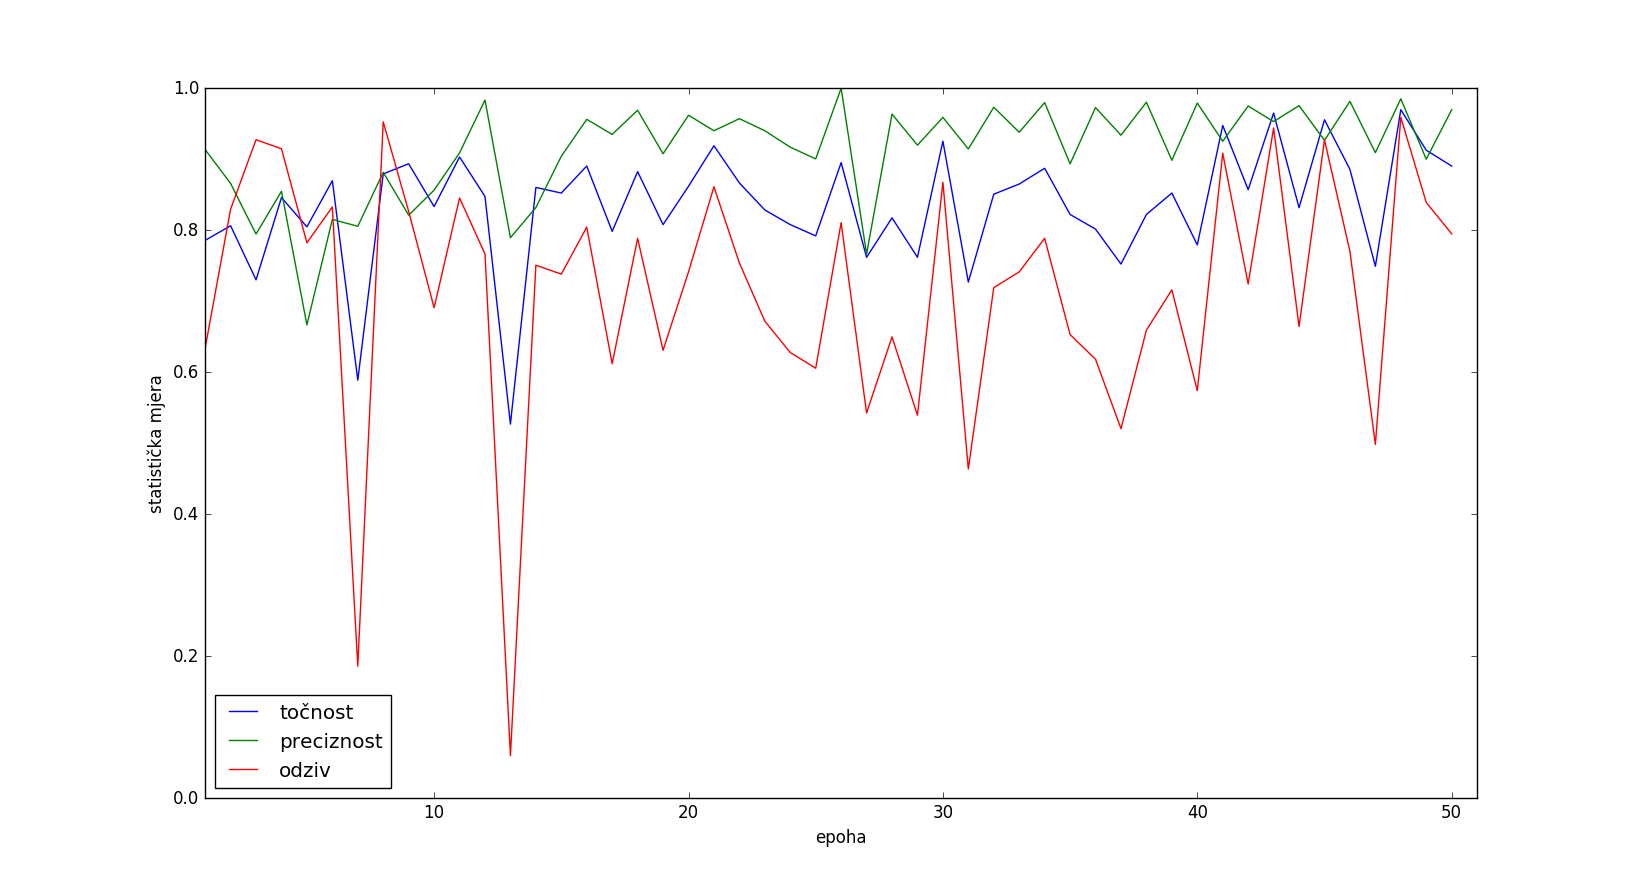
\includegraphics[scale=0.35]{images/single_hand_scale1_acc_ap.png}
\caption{Kretanje točnosti, preciznosti i odziva na podskupu za validaciju po epohama}
\label{img:single_hand_scale1_acc_ap}
\end{figure}
\noindent Na slici \ref{img:single_hand_scale1_acc_ap} vidljivo je kretanje točnosti, preciznosti i odziva po epohama na podskupu za validaciju.

\subsection{Rezultati na rezoluciji 525x210}
Konačni rezultati dobiveni za eksperiment s ulaznim podacima rezolucije $525$x$210$ su sljedeći:
\begin{table}[H]
\centering
\caption{Statistički rezultati na rezoluciji $525$x$210$}
\label{score:single_hand_525x210}
\begin{tabular}{|c|c|c|c|c|}
\hline
podskup podataka      & točnost & preciznost & odziv & prosječna preciznost \\ \hline
podskup za učenje     & 1.0     & 1.0        & 1.0   & 1.0\\ \hline
podskup za validaciju & 0.92     & 0.99        & 0.85  & 0.99 \\ \hline
podskup za testiranje & 0.98     & 0.99          & 0.96  & 0.99 \\ \hline
\end{tabular}
\end{table}
\begin{table}[H]
\centering
\caption{Odnos predikcija modela i stvarnih oznaka na rezoluciji $525$x$210$ na podskupu za učenje}
\label{score:single_hand_525x210_tpfptnfn_train}
\begin{tabular}{|c|c|c|}
\hline
\diagbox{stvarna oznaka}{predikcija modela} & 0  & 1  \\ \hline
0                                & 898 & 0 \\ \hline
1                                & 0 & 898 \\ \hline
\end{tabular}
\end{table}
\begin{table}[H]
\centering
\caption{Odnos predikcija modela i stvarnih oznaka na rezoluciji $525$x$210$ na podskupu za validaciju}
\label{score:single_hand_525x210_tpfptnfn_valid}
\begin{tabular}{|c|c|c|}
\hline
\diagbox{stvarna oznaka}{predikcija modela} & 0  & 1  \\ \hline
0                                & 310 & 3 \\ \hline
1                                & 48 & 265 \\ \hline
\end{tabular}
\end{table}
\begin{table}[H]
\centering
\caption{Odnos predikcija modela i stvarnih oznaka na rezoluciji $525$x$210$ na podskupu za testiranje}
\label{score:single_hand_525x210_tpfptnfn_test}
\begin{tabular}{|c|c|c|}
\hline
\diagbox{stvarna oznaka}{predikcija modela} & 0  & 1  \\ \hline
0                                & 295 & 2 \\ \hline
1                                & 12 & 285 \\ \hline
\end{tabular}
\end{table}
\noindent Tablica \ref{score:single_hand_525x210} prikazuje rezultate dobivene evaluacijom modela koji je postigao najbolju performansu na podskupu za validaciju prilikom učenja.
Tablice \ref{score:single_hand_525x210_tpfptnfn_train}, \ref{score:single_hand_525x210_tpfptnfn_valid} i \ref{score:single_hand_525x210_tpfptnfn_test} prikazuju odnos predikcija modela i stvarnih oznaka kroz matricu zabune.

\begin{figure}[H]
\centering
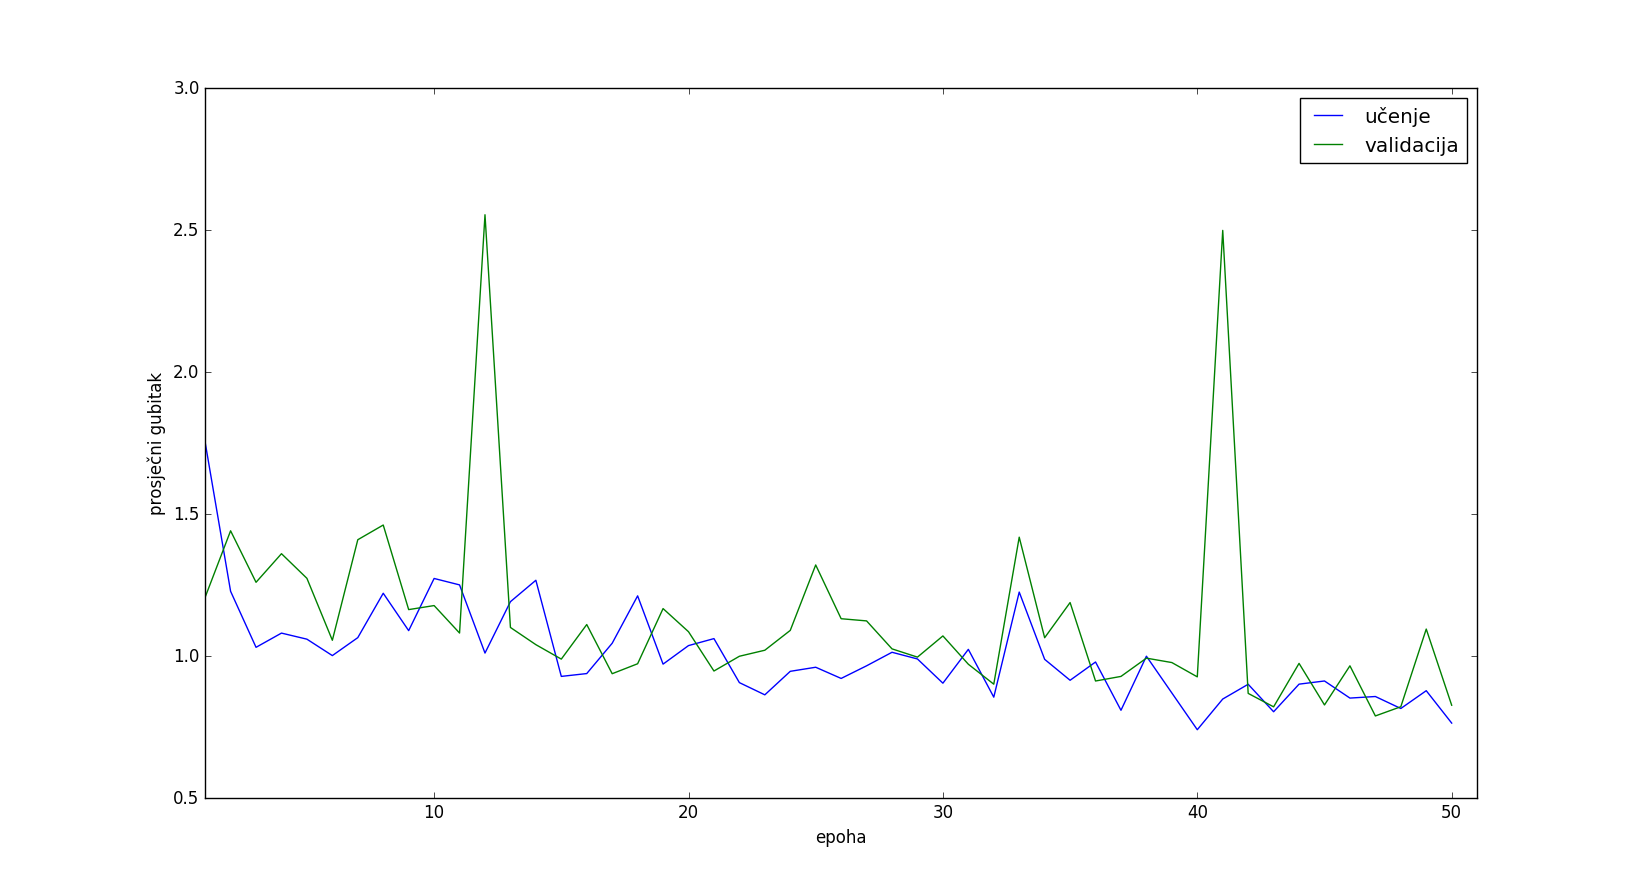
\includegraphics[scale=0.35]{images/single_hand_scale075_loss.png}
\caption{Kretanje prosječnog gubitka na podskupu za učenje i validaciju po epohama}
\label{img:single_hand_scale075_loss}
\end{figure}
\noindent Na slici \ref{img:single_hand_scale075_loss} vidljivo je kretanje prosječnog gubitka po epohama na podskupu za učenje i na podskupu za validaciju.

\begin{figure}[H]
\centering
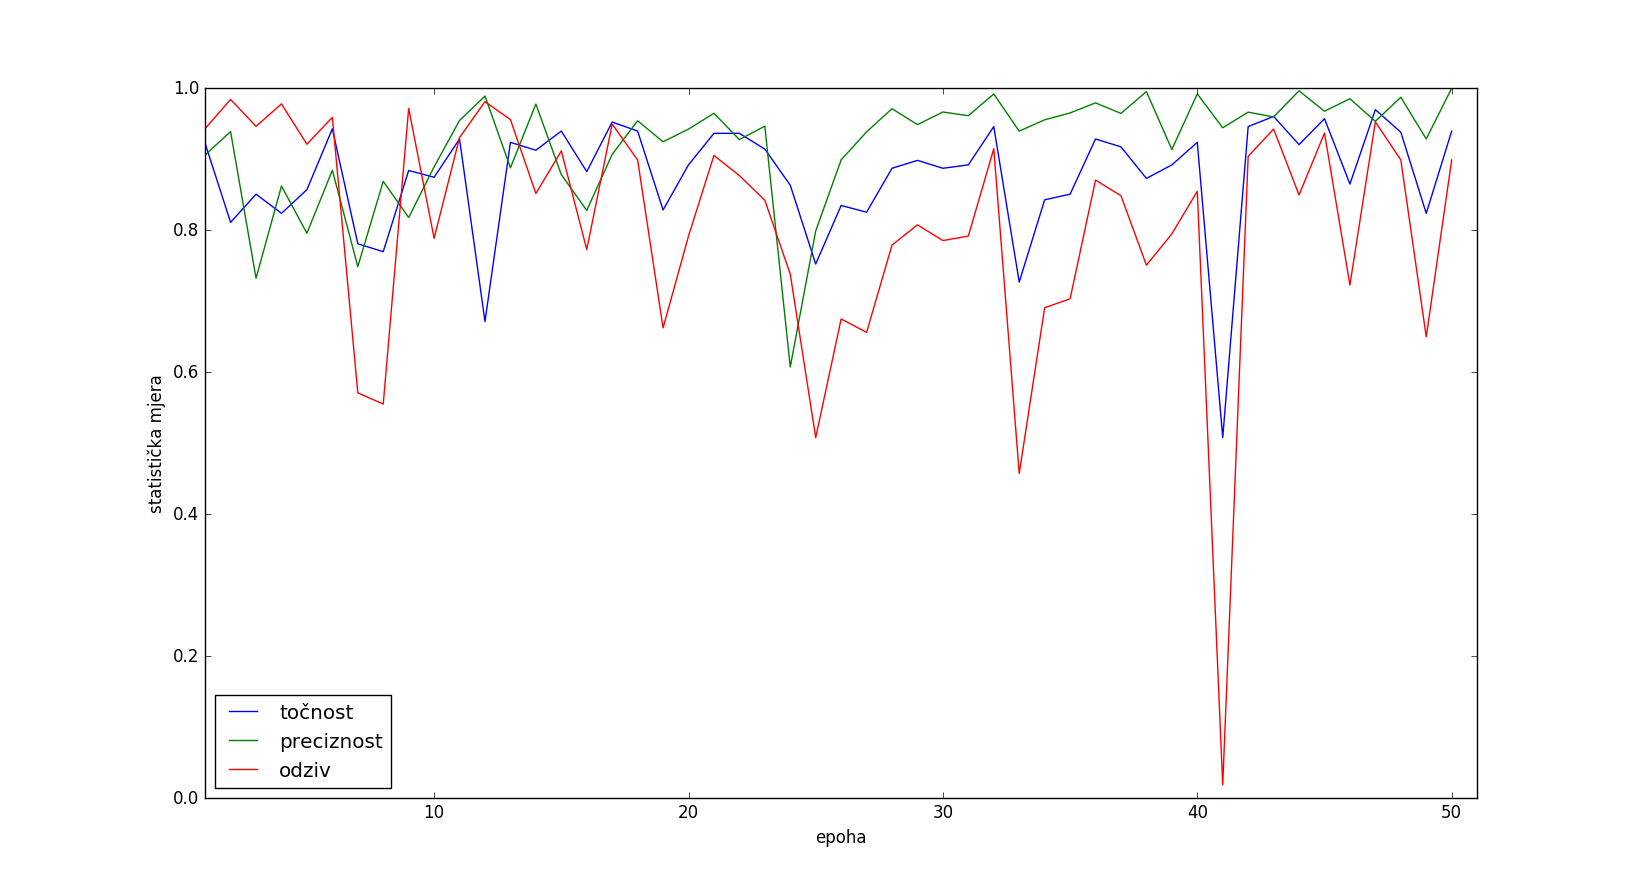
\includegraphics[scale=0.35]{images/single_hand_scale075_acc_ap.png}
\caption{Kretanje točnosti, preciznosti i odziva po epohama}
\label{img:single_hand_scale075_acc_ap}
\end{figure}
\noindent Na slici \ref{img:single_hand_scale075_acc_ap} vidljivo je kretanje točnosti, preciznosti i odziva po epohama na podskupu za validaciju.

\subsection{Rezultati na rezoluciji 350x140}
Konačni rezultati dobiveni za eksperiment s ulaznim podacima rezolucije $350$x$140$ su sljedeći:
\begin{table}[H]
\centering
\caption{Statistički rezultati na rezoluciji  $350$x$140$}
\label{score:single_hand_350x140}
\begin{tabular}{|c|c|c|c|c|}
\hline
podskup podataka      & točnost & preciznost & odziv & prosječna preciznost \\ \hline
podskup za učenje     & 1.0     & 1.0        & 1.0  & 1.0 \\ \hline
podskup za validaciju & 0.92     & 0.96        & 0.88 &  0.99 \\ \hline
podskup za testiranje & 0.98     & 0.96          & 0.99 &  0.99 \\ \hline
\end{tabular}
\end{table}
\begin{table}[H]
\centering
\caption{Odnos predikcija modela i stvarnih oznaka na rezoluciji  $350$x$140$ na podskupu za treniranje}
\label{score:single_hand_350x140_tpfptnfn_train}
\begin{tabular}{|c|c|c|}
\hline
\diagbox{stvarna oznaka}{predikcija modela} & 0  & 1  \\ \hline
0                                & 898 & 0 \\ \hline
1                                & 0 & 898 \\ \hline
\end{tabular}
\end{table}
\begin{table}[H]
\centering
\caption{Odnos predikcija modela i stvarnih oznaka na rezoluciji  $350$x$140$ na podskupu za validaciju}
\label{score:single_hand_350x140_tpfptnfn_valid}
\begin{tabular}{|c|c|c|}
\hline
\diagbox{stvarna oznaka}{predikcija modela} & 0  & 1  \\ \hline
0                                & 303 & 10 \\ \hline
1                                & 39 & 274 \\ \hline
\end{tabular}
\end{table}
\begin{table}[H]
\centering
\caption{Odnos predikcija modela i stvarnih oznaka na rezoluciji  $350$x$140$ na podskupu za testiranje}
\label{score:single_hand_350x140_tpfptnfn_test}
\begin{tabular}{|c|c|c|}
\hline
\diagbox{stvarna oznaka}{predikcija modela} & 0  & 1  \\ \hline
0                                & 286 & 11 \\ \hline
1                                & 2 & 295 \\ \hline
\end{tabular}
\end{table}
\noindent Tablica \ref{score:single_hand_350x140} prikazuje rezultate dobivene evaluacijom modela koji je postigao najbolju performansu na podskupu za validaciju prilikom učenja.
Tablice \ref{score:single_hand_350x140_tpfptnfn_train}, \ref{score:single_hand_350x140_tpfptnfn_valid} i \ref{score:single_hand_350x140_tpfptnfn_test} prikazuju odnos predikcija modela i stvarnih oznaka kroz matricu zabune.

\begin{figure}[H]
\centering
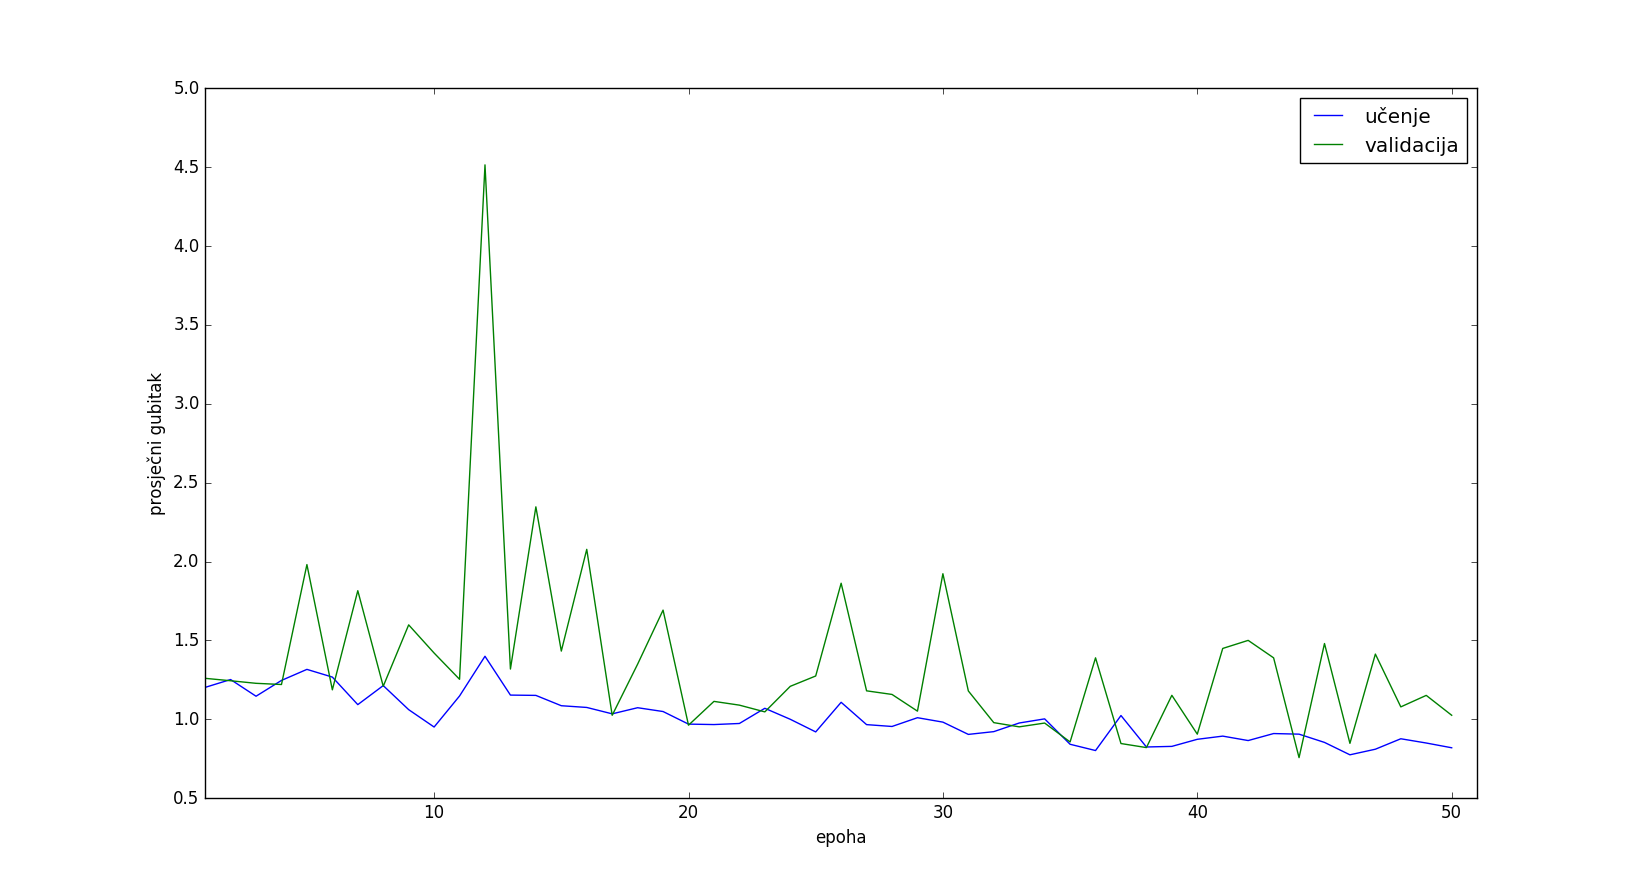
\includegraphics[scale=0.35]{images/single_hand_scale050_loss.png}
\caption{Kretanje prosječnog gubitka na podskupu za učenje i validaciju po epohama}
\label{img:single_hand_scale050_loss}
\end{figure}
\noindent Na slici \ref{img:single_hand_scale050_loss} vidljivo je kretanje prosječnog gubitka po epohama na podskupu za učenje i na podskupu za validaciju.

\begin{figure}[H]
\centering
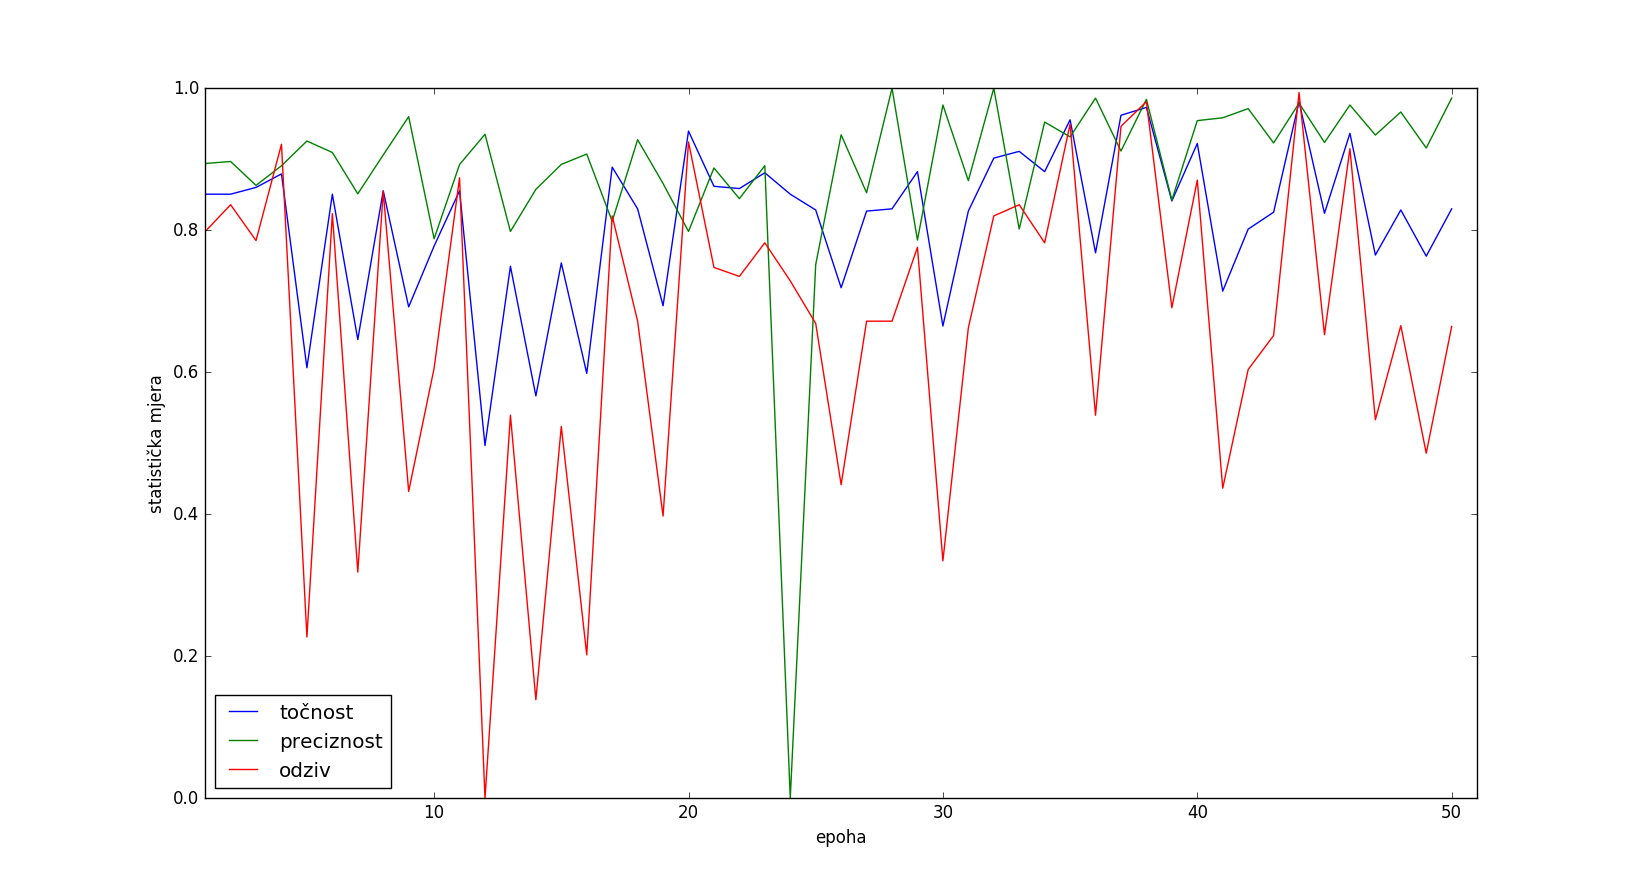
\includegraphics[scale=0.35]{images/single_hand_scale050_acc_ap.png}
\caption{Kretanje točnosti, preciznosti i odziva na podskupu za validaciju po epohama}
\label{img:single_hand_scale050_acc_ap}
\end{figure}
\noindent Na slici \ref{img:single_hand_scale050_acc_ap} vidljivo je kretanje točnosti, preciznosti i odziva po epohama na podskupu za validaciju.

\subsection{Rezultati na rezoluciji 175x70}
Konačni rezultati dobiveni za eksperiment s ulaznim podacima rezolucije $175$x$70$ su sljedeći:
\begin{table}[H]
\centering
\caption{Statistički rezultati na rezoluciji $175$x$70$}
\label{score:single_hand_175x70}
\begin{tabular}{|c|c|c|c|c|}
\hline
podskup podataka      & točnost & preciznost & odziv & prosječna preciznost \\ \hline
podskup za učenje     & 1.0     & 1.0        & 1.0  & 1.0  \\ \hline
podskup za validaciju & 0.81     & 0.98        & 0.63  & 0.96 \\ \hline
podskup za testiranje & 0.71     & 0.96          & 0.43 & 0.92 \\ \hline
\end{tabular}
\end{table}
\begin{table}[H]
\centering
\caption{Odnos predikcija modela i stvarnih oznaka na rezoluciji $175$x$70$ na podskupu za učenje}
\label{score:single_hand_175x70_tpfptnfn_train}
\begin{tabular}{|c|c|c|}
\hline
\diagbox{stvarna oznaka}{predikcija modela} & 0  & 1  \\ \hline
0                                & 898 & 0 \\ \hline
1                                & 0 & 898 \\ \hline
\end{tabular}
\end{table}
\begin{table}[H]
\centering
\caption{Odnos predikcija modela i stvarnih oznaka na rezoluciji $175$x$70$ na podskupu za validaciju}
\label{score:single_hand_175x70_tpfptnfn_valid}
\begin{tabular}{|c|c|c|}
\hline
\diagbox{stvarna oznaka}{predikcija modela} & 0  & 1  \\ \hline
0                                & 310 & 3 \\ \hline
1                                & 117 & 196 \\ \hline
\end{tabular}
\end{table}
\begin{table}[H]
\centering
\caption{Odnos predikcija modela i stvarnih oznaka na rezoluciji $175$x$70$ na podskupu za testiranje}
\label{score:single_hand_175x70_tpfptnfn_test}
\begin{tabular}{|c|c|c|}
\hline
\diagbox{stvarna oznaka}{predikcija modela} & 0  & 1  \\ \hline
0                                & 291 & 6 \\ \hline
1                                & 169 & 128 \\ \hline
\end{tabular}
\end{table}
\noindent Tablica \ref{score:single_hand_175x70} prikazuje rezultate dobivene evaluacijom modela koji je postigao najbolju performansu na podskupu za validaciju prilikom učenja.
Tablice \ref{score:single_hand_175x70_tpfptnfn_train}, \ref{score:single_hand_175x70_tpfptnfn_valid} i \ref{score:single_hand_175x70_tpfptnfn_test} prikazuju odnos predikcija modela i stvarnih oznaka kroz matricu zabune.

\begin{figure}[H]
\centering
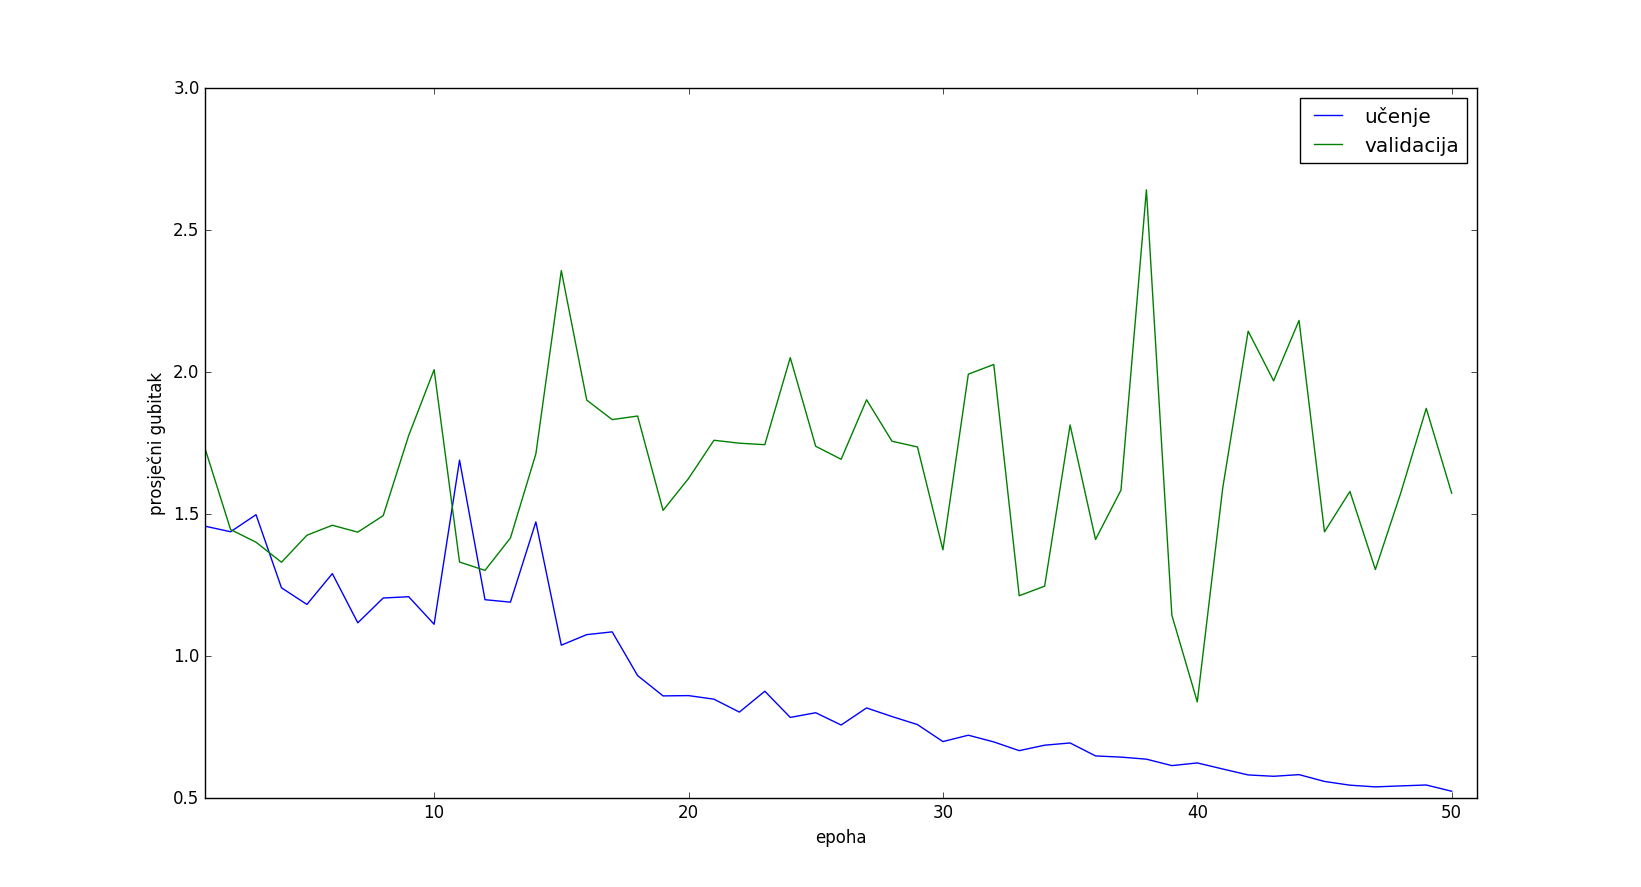
\includegraphics[scale=0.35]{images/single_hand_scale025_loss.png}
\caption{Kretanje prosječnog gubitka na skupu za učenje i validaciju po epohama}
\label{img:single_hand_scale025_loss}
\end{figure}
\noindent Na slici \ref{img:single_hand_scale025_loss} vidljivo je kretanje prosječnog gubitka po epohama na podskupu za učenje i na podskupu za validaciju.

\begin{figure}[H]
\centering
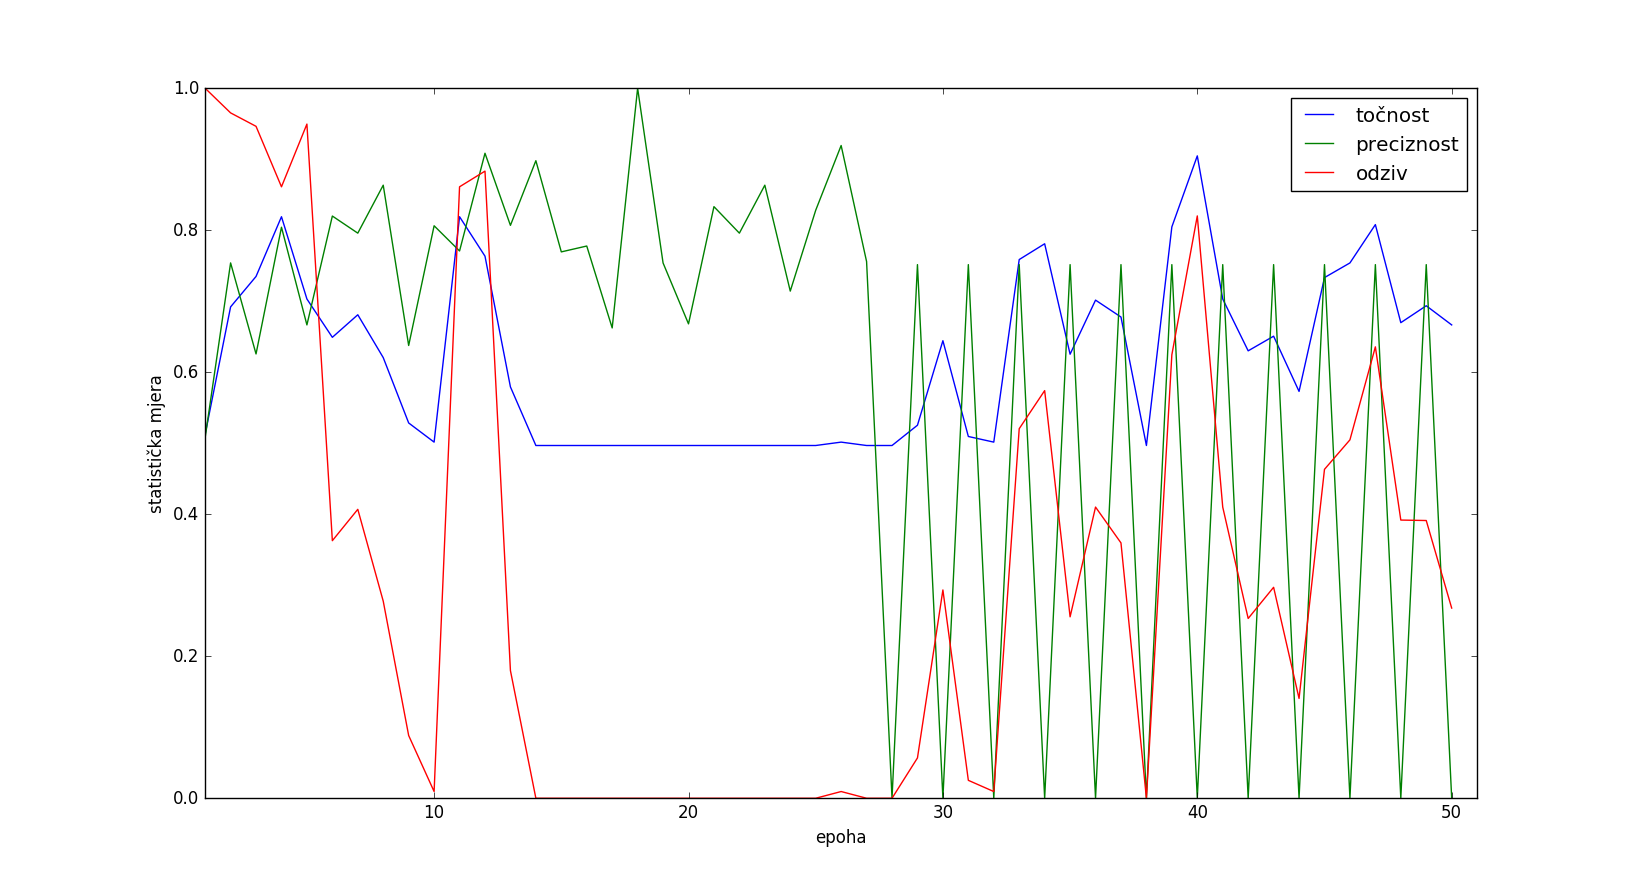
\includegraphics[scale=0.35]{images/single_hand_scale025_acc_ap.png}
\caption{Kretanje točnosti, preciznosti i odziva po epohama}
\label{img:single_hand_scale025_acc_ap}
\end{figure}
\noindent Na slici \ref{img:single_hand_scale025_acc_ap} vidljivo je kretanje točnosti, preciznosti i odziva po epohama na podskupu za validaciju.

Vidljivo je kako se tek na rezoluciji $175$x$70$ pojavljuje značajniji pad performansi. 
Iz tog razloga se za eksperimente nad sekvencama slika (zbog veće memorijske zahtjevnosti) koriste rezolucije pojedinih slika $350$x$140$.

\section{Klasifikacija pojedinačnih slika označenih konzistentno s projektom FTTS iRAP na originalnoj rezoluciji}
Za razliku od prethodnih eksperimenata, ovaj eksperiment je proveden na skupu podataka označenom konzistentno sa sustavom FTTS iRAP.
Eksperiment je proveden na pojedinačnim slikama kako bi se u daljnjim eksperimentima moglo usporediti poboljšava li se rezultat uvođenjem dodatnih informacija sa sekvencom slika koje prethode slici za koju je određena oznaka prisutnosti atributa pripajanja.

\section{Klasifikacija sekvenci slika označenih konzistentno s projektom FTTS iRAP koristeći vremensko-prostorno sažimanje}
Konačni rezultati dobiveni za eksperiment sa sekvencijalnim ulaznim podacima rezolucije $350$x$140$ su sljedeći:
\begin{table}[H]
\centering
\caption{Statistički rezultati}
\label{score:single_hand_175x70}
\begin{tabular}{|c|c|c|c|c|}
\hline
podskup podataka      & točnost & preciznost & odziv & prosječna preciznost \\ \hline
podskup za učenje     & 1.0     & 1.0        & 1.0  & 1.0  \\ \hline
podskup za validaciju & 0.81     & 0.98        & 0.63  & 0.96 \\ \hline
podskup za testiranje & 0.71     & 0.96          & 0.43 & 0.92 \\ \hline
\end{tabular}
\end{table}
\begin{table}[H]
\centering
\caption{Odnos predikcija modela i stvarnih oznaka na rezoluciji $175$x$70$ na podskupu za učenje}
\label{score:single_hand_175x70_tpfptnfn_train}
\begin{tabular}{|c|c|c|}
\hline
\diagbox{stvarna oznaka}{predikcija modela} & 0  & 1  \\ \hline
0                                & 898 & 0 \\ \hline
1                                & 0 & 898 \\ \hline
\end{tabular}
\end{table}
\begin{table}[H]
\centering
\caption{Odnos predikcija modela i stvarnih oznaka na rezoluciji $175$x$70$ na podskupu za validaciju}
\label{score:single_hand_175x70_tpfptnfn_valid}
\begin{tabular}{|c|c|c|}
\hline
\diagbox{stvarna oznaka}{predikcija modela} & 0  & 1  \\ \hline
0                                & 310 & 3 \\ \hline
1                                & 117 & 196 \\ \hline
\end{tabular}
\end{table}
\begin{table}[H]
\centering
\caption{Odnos predikcija modela i stvarnih oznaka na rezoluciji $175$x$70$ na podskupu za testiranje}
\label{score:single_hand_175x70_tpfptnfn_test}
\begin{tabular}{|c|c|c|}
\hline
\diagbox{stvarna oznaka}{predikcija modela} & 0  & 1  \\ \hline
0                                & 291 & 6 \\ \hline
1                                & 169 & 128 \\ \hline
\end{tabular}
\end{table}
\noindent Tablica \ref{score:single_hand_175x70} prikazuje rezultate dobivene evaluacijom modela koji je postigao najbolju performansu na podskupu za validaciju prilikom učenja.
Tablice \ref{score:single_hand_175x70_tpfptnfn_train}, \ref{score:single_hand_175x70_tpfptnfn_valid} i \ref{score:single_hand_175x70_tpfptnfn_test} prikazuju odnos predikcija modela i stvarnih oznaka kroz matricu zabune.

\begin{figure}[H]
\centering
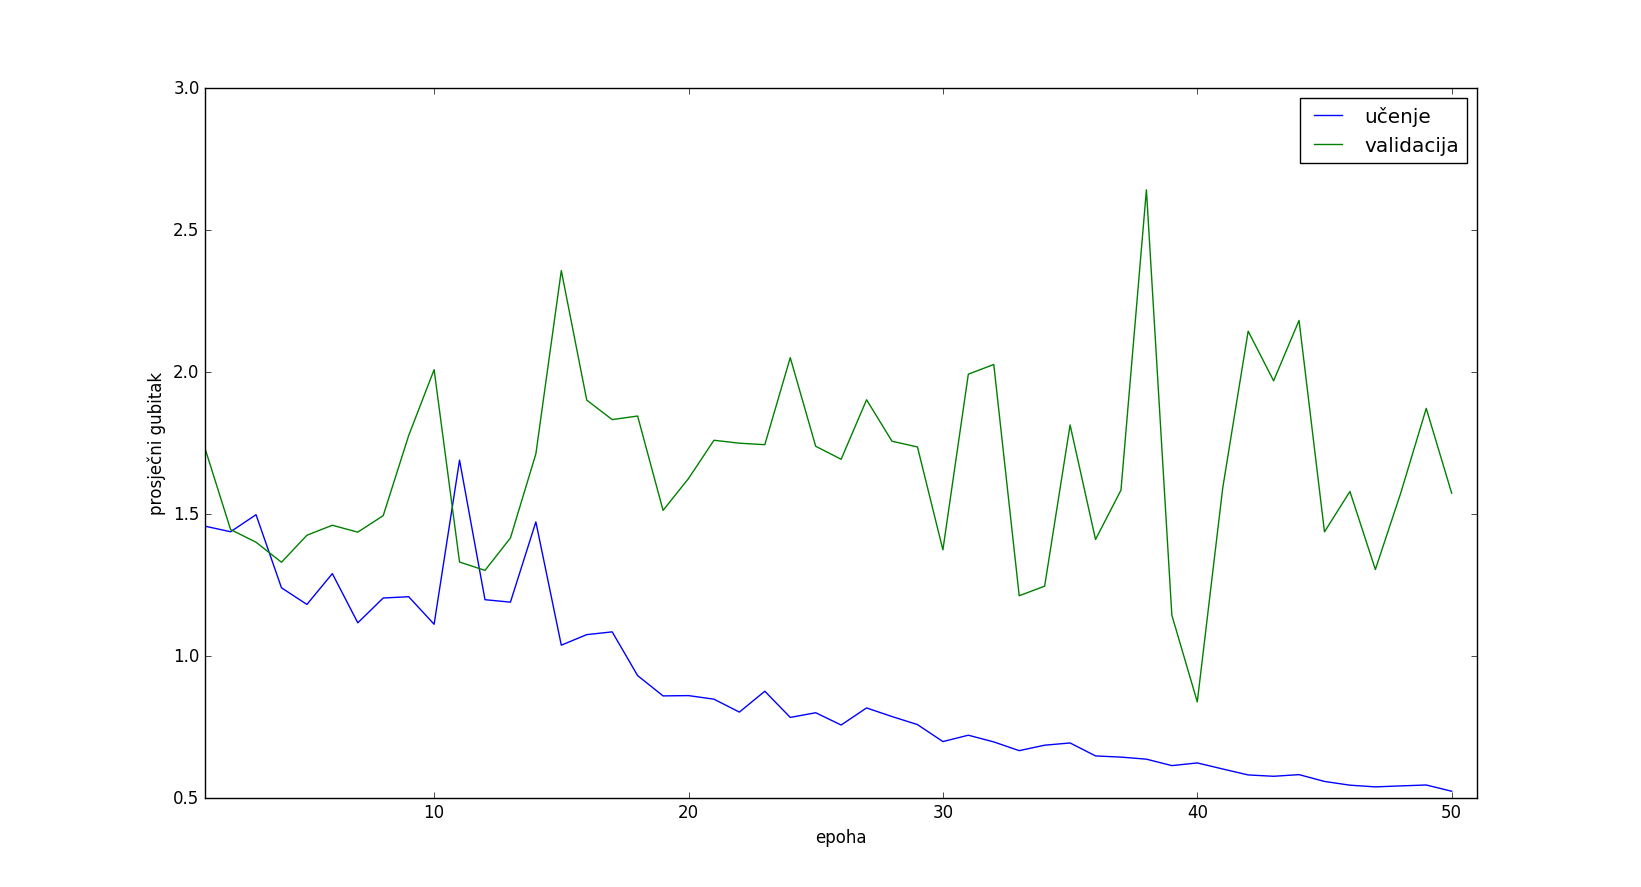
\includegraphics[scale=0.35]{images/single_hand_scale025_loss.png}
\caption{Kretanje prosječnog gubitka na skupu za učenje i validaciju po epohama}
\label{img:single_hand_scale025_loss}
\end{figure}
\noindent Na slici \ref{img:single_hand_scale025_loss} vidljivo je kretanje prosječnog gubitka po epohama na podskupu za učenje i na podskupu za validaciju.

\begin{figure}[H]
\centering
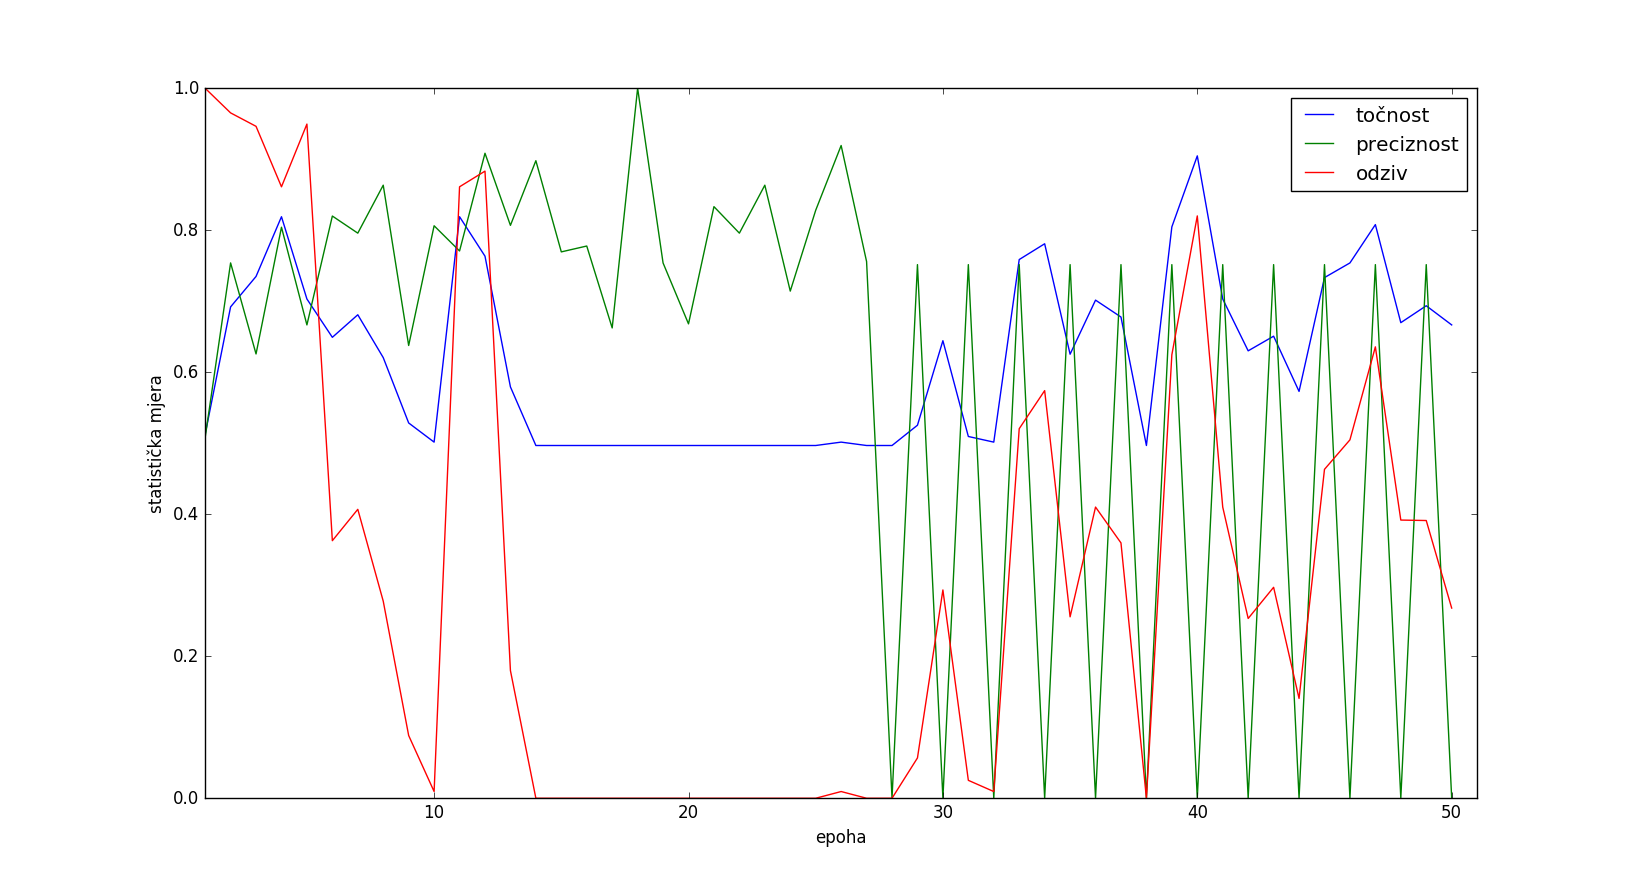
\includegraphics[scale=0.35]{images/single_hand_scale025_acc_ap.png}
\caption{Kretanje točnosti, preciznosti i odziva po epohama}
\label{img:single_hand_scale025_acc_ap}
\end{figure}
\noindent Na slici \ref{img:single_hand_scale025_acc_ap} vidljivo je kretanje točnosti, preciznosti i odziva po epohama na podskupu za validaciju.

Vidljivo je kako se tek na rezoluciji $175$x$70$ pojavljuje značajniji pad performansi. 
Iz tog razloga se za eksperimente nad sekvencama slika (zbog veće memorijske zahtjevnosti) koriste rezolucije pojedinih slika $350$x$140$.

\section{Klasifikacija sekvenci slika označenih konzistentno s projektom FTTS iRAP koristeći povratne LSTM ćelije}

\section{Klasifikacija sekvenci slika označenih konzistentno s projektom FTTS iRAP koristeći vremenski potpuno povezani sloj}

\section{Analiza rezultata}

\chapter{Zaključak}
Zaključak.

\bibliography{literatura}
\bibliographystyle{fer}

\begin{sazetak}
Sažetak na hrvatskom jeziku.

\kljucnerijeci{Ključne riječi, odvojene zarezima.}
\end{sazetak}

% TODO: Navedite naslov na engleskom jeziku.
\engtitle{Title}
\begin{abstract}
Abstract.

\keywords{Keywords.}
\end{abstract}

\end{document}
